% Motivation
    %% Coating Thermal Noise
	%%% Brownian Thermal Noise
	    %%%% Internal Friction in Materials and Loss Angle
    	    %%%% Coating Brownian Thermal Noise
    	    %%%% Silica Ti-Tantala coating parameters
    	    %%%% GaAs/AlGaAs coating parameters
    %% Anisotropic Media
	%%% The Dielectric Tensor
    	%%% Indicatrix
    	%%% Linear Electro-optic Effect (Pockel's Effect)
    	%%% Electro-optic coefficients r_ij for zincblende crystals
    	%%% New Principal (electro-optic) dielectric constants for zincblende structures
    	%%% The photoelastic effect
    	%%% The generalized indicatrix
    %% EO modulation
    %% Optical anisotropy of an HR GaAs / AlGaAs stack
    %% Miller indices for HR GaAs / AlGaAs coatings
        %%% Electro-optic coupling to the reflected phase of a HR mirror coating
    %% Numerical estimate
    %% Measured birefringence from HR \texorpdfstring{$\gaas$}{gaas}/\texorpdfstring{$\algaas$}{algaas} mirrors
    %% Initial projected DARM coupling

% Electro-optic measurement apparatus
    %% PDH servo
    %% Servo Parameters
	%%% Sensing S(f)
    	%%% Actuation A(f)
    	%%% Low Frequency Servo (Thermal Loop)
    	%%% OLG(f) 
    %% Longitudinal Pockels Cell mirror mount assembly
	%%% Modeling
    	%%% Voltage drive electronics
    %% Servo Overview
    %% Calibration

% Results
    %% Mounting Strategies
	%%% Assembly 1
    	%%% Assembly 2
    	%%% Assembly 3 (MACOR mount)
    	%%% Acousto-optical coupling

% Conclusion

As mentioned in \autoref{subsubsec:introctn}, once mirror coating materials are selected for DRFPMI core optics, another fundamental detector noise limit is simultaneously imposed. As aLIGO approaches designed sensitivity, there are efforts proposing the usage of alternative mirror coating solutions, with the primary purpose of pushing down the thermal noise limit and further enhancing detector sensitivity \cite{harry:aigwd2019}. $\gaas$/$\algaas$ shows promise for next generation detectors with reduced coating Brownian noise by a factor of 10, cooresponding to a potential strain reduction by a factor of 5 ~\cite{cole:2013} when compared to the current aLIGO coating thermal noise limit. Though applying crystalline HR mirror coatings to the core optics does introduce notable side effects; one being linear electro-optic of $\gaas$/$\algaas$ (dn/dE), also known as the Pockels effect ~\cite{abernathy:poster}. A differential phase noise estimate of $\approx 10^{-11}$ [rad/m/V], alongside measured ambient field noise of $3\times 10^{-6}$ [V/m/$\sqrt{\mathrm{Hz}}$] presents adequate motivation for a thorough study dedicated to the electro-optical properties of $\gaas$/$\algaas$ coatings~\cite{buikema:2020}. This section details such a study that starts with a brief survey of the optical and material properties of crystalline materials like $\gaas$ and $\algaas$ by reviewing: light propogation through anistropic materials, and induced optical anisotropy of zincblende materials. The second item of discussion are preliminary estimates of the differential phase of light reflected from a $\gaas$/$\algaas$ coating stack caused by electric field noise are computed while considering potential impacts to the current generation gravitational wave detectors. The third and final item of discussion is a study designed to acquire dn/dE estimates from a calibrated differential length PDH locked signal from a short experimental optical cavity with a primarily normal electric field driven across a HR $\gaas$/$\algaas$ coating ``witness" sample.

\section{Motivation}

\subsection{Coating Thermal Noise}
Contributions of categorized noises for gravitational wave detectors are organized in a ``noise budget", comprised of a collection of technical (noise imposed by the practical operation of the detector) and fundamental (inherent physical limitations of DRFPMIs by design) noise sources that impose limitations on gravitational wave detection.
%% Contributions of categorized noises for gravitational wave detectors the ''noise budget" ((LHO and LLO O3?) or just GWINC?)}

\subsubsection{Brownian Thermal Noise}
%% Might move this section back to the $\algaas$ Electro-optic noise chapter
In 1827 the Scottish botanist Robert Brown noticed a constant motion of pollen particulates on the surface of water; witnessing randomized collisions of the water molecules holding a kinetic energy proportional to the temperature ($k_BT$) \cite{brown:1828}. It is because of his documented observations we name the phenomena Brownian motion. And although the observations were on motion of particulates in liquids, molecules and atoms within gases and solids also exhibit Brownian motion. For high precision optical experiments operating at room temperature (and higher due to high power resonant beams), understanding how much differential phase noise is imparted on the interferometer light passing through and reflecting from core optics is crucial. This requires knowledge of the mean squared displacement from each degree of freedom of the system which can be realized through the Fluctuation Dissapation theorem. Derived by H.B. Callen and T.A. Welton, the theorem states that for a randomly fluctuating linear force \cite{callen:1951}:

%% Further insight into Brownian motion was explored by Einstein where he was able to relate the mean-square displacement of a particle of radius $r_\mathrm{sph}$ on a fluid with viscosity $\eta$.
 %%\begin{equation}
 %%\overline{x^2} = k_B T  \frac{1}{3 \pi \eta  r_\mathrm{sph}}
 %%\end{equation}
 %%This relation has important implications about how the random motion or fluctuations of a particulate (the pollen) is influenced (dissipated) by the viscosity of the surrounding medium (water).

\begin{equation}
F_x^2(f) = 4 k_B T\; \Re[Z]
\end{equation}

 \noindent Where $\Re[Z]$ is the real part of the impedance of the system. This impedance directly relates to equations of motion:

 \begin{equation}
 Z = \frac{F}{\dot{x}}
 \end{equation}

\noindent Another useful form is the power spectrum of the fluctuating motion:
\begin{equation}\label{eq:fdtpsd}
x^2 (f)  = \frac{4k_B T}{(2 \pi f)^2}\; \Re[Y]
\end{equation}

Where $Y$ is the inverse impedance or admittance. $x^2(f)$ as informed by the FDT facilitates modelling and budgeting notable LIGO fundamental noise contributions made by choice of materials used for mirror substrates and highly reflective mirror coatings. Though adequate modelling of internal force couplings for the aforementioned components provides a more complete picture.

\paragraph{Internal friction in Materials and Loss angle}

Zener provides a model of the internal friction of materials incorporating anelasticity into the equations of motion \cite{zener:1948}:

\begin{equation}
F = k(1+i\phi)x + m\ddot{x}
\end{equation}

Where $m$ is mass attached to a spring with a spring constant $k(1+ i\phi)$ incorporating the degree of anelasticity $\phi$. From equations 3.5 and 3.3 we perform a Laplace transform and acquire the following form of admittance:
\begin{equation}
Y(s) = \frac{\dot{x}(s)}{F(s)} = \frac{-s}{k(1+i\phi) + ms^2}
\end{equation}

\noindent Or more transparently the Fourier representation since we assume a linear time invariant system:

\begin{equation}\label{eq:admitint}
Y(\omega) = \frac{\dot{x}(\omega)}{F(\omega)} = \frac{-i\omega}{k(1+i\phi) - m\omega^2} = \frac{k \omega \phi - i \omega (k - m \omega^2)}{(k-m\omega^2)^2 +k^2 \phi^2}
\end{equation}

\noindent Plugging equation \autoref{eq:admitint} back into \autoref{eq:fdtpsd}:

\begin{equation}
x^2 (f)  = \frac{2k_B T}{\pi}\frac{k\phi}{(k-4\pi^2 m f^2)^2 + k^2 \phi^2}
\end{equation}

Computing the admittance from a Gaussian beam impinging upon a HR mirror can require expansion of all individual mechanical degrees of freedom of the test mass system across a relevant frequency range, and with that approach convergence is not guaranteed. Saulson and Gonzalez provide an alternative method to computing the admittance coined the ``direct approach" by Levin when computing the noise from a Gaussian beam on a LIGO HR test mass. The admittance can be acquired through:

\begin{equation}\label{eq:admitdirec}
\Re[Y] = \frac{W_\mathrm{diss}}{F_o^2}
\end{equation}

\noindent $W_\mathrm{diss}$ is the dissipated power from the system due to an oscillating force $F_o$. This form of the admittance reveals an important result of the fluctuation dissapation theorem where an undriven system with a dissapative actor, imparts motion to the degrees of freedom via a driving force by virtue of that same actor at finite temperatures. This direct approach also allows the surface pressure applied by the Gaussian beam to interrogate which mechanical modes of the test mass impose a significant energy when \autoref{eq:admitdirec} is plugged into \autoref{eq:fdtpsd}. In the case of the gaussian beam / uncoated test mass studied by Levin \cite{levin:1998}:

\begin{equation}
S_x(f) = \frac{4 k_B T}{f} \frac{1-\sigma^2}{\pi^3 E_o r_o} I\phi \bigg[1- O\bigg( \frac{r_o}{R} \bigg)\bigg]
\end{equation}

%this requires that the driving force used in a lab mimics that of a force from a centered Gaussian beam.

%%Refer to Levin appendix for more on how elasticity parameters are introduced?
Where $\phi$ and $E_o$ are the Poisson ratio and Young's modulus respectively, and $O(\frac{r_o}{R})$ contains a correction term contribution as a function of the small beam radius ($r_o$) relative to the mirror radius ($R$).

\paragraph{Coating Brownian thermal noise}
Further investigations into the beam/optic system utilizing this approach and elasticity theory led to a deeper understanding about Brownian thermal noise contributions from LIGO test masses (substrate, suspensions, HR coating). Levin mentions, with details from Harry, that the noise contributed by a lossy mirror coating is proven to be to be the most significant contributor of brownian thermal noise. Hong provides a power spectral density \cite{hong:2013}:

\begin{equation}
S_j^X = \frac{4k_B T \lambda \phi_x^j(1- \sigma_j - 2 \sigma_j^2)}{3 \pi^2 f Y_j (1-\sigma_j)^2 \omega_o^2}
\end{equation}

Where X represents bulk and shear with j = odd (material 1) and j = even (material 2) alternating layers representing high and low index materials j = odd (material 1) j = even (material 2) for an HR coating.

\begin{figure}[H]
    \begin{center}
    \includegraphics[width=.9\textwidth]{ALGAAS/aligo_nb_plus_cbn.pdf}
    \end{center}
    \caption{ALIGO noise budget placeholder for silica-tantala, and gaas-algaas brownian noise comparison}
\label{fig:aligotncomp}
\end{figure}

\paragraph{$\siotao$ coating parameters}
Currently the LIGO interferometers deposit $\lambda$/4 stacks of silica and titania doped tantala on fused silica test mass substrates. Effective loss angle measurements \cite{harry:2006}

\textbf{Current $\siotao$ elasticity params, power spectra, and strain spectral density (order of magnitude estimate)}

\paragraph{$\gaas$/$\algaas$ coating parameters}
%%Specific coating parameters for most promising $\algaas$ candidates? Chat with Steve. Or just mention parameters that are listed in Cole 2013
\cite{cole:2013}

%% Insert computed curves of the most precise and recent (effective) loss angle measurements (Nick Demos measurements?). More instructive to plot strain spectral density or displacement power spectra

\noindent Currently thermal noise from the $\siotao$ optical coatings is the largest contributor of Brownian noise in LIGO compared to estimated substrate and suspension thermal noise \cite{harry:2006}. As of the end of O3, Brownian thermal noise is estimated to be ? orders of magnitude below the current sensitivity and it will prove to be the limiting source of noise as that sensitivity is increased with various other upgrades mitigating fundamental and technical noise. 
%% Already mentioned in intro prior to this thermal noise section. Need to re-iterate in more detail?

\subsection{Anisotropic media}
Unlike isotropic media, we do not assume that the index of refraction of anisotropic media is the same for all chosen wave vectors. This is a direct consequence of the birefringence of anisotropic media; characterized by the dielectric, permittivity, and polarization tensors.

\subsubsection{The Dielectric tensor}
Further elaborating on the nature of a generalized dielectric tensor ($\varepsilon$) for any wavevector is required to proceed:
\begin{equation}\label{eq:dispfield}
D_i = \varepsilon_{ij}E_j
\end{equation}
Where D is the displacement vector, E is the electric field vector, and $\varepsilon$ is the dielectric tensor. The displacement vector for isotropic media is retrieved when $i = j$ and $\varepsilon_i = \varepsilon$. To further understand the nature of the dielectric tensor we assert Poynting's theorem providing an energy conservation requirement:
\begin{equation}\label{eq:poynting}
\nabla \cdot \vec{S} = \frac{dU}{dt}
\end{equation}
Where $\vec{S} = \vec{E} \times \vec{H}$ is the poynting vector and $U = \frac{1}{8 \pi} \big( \vec{E} \cdot \vec{D} + \vec{B} \cdot \vec{H} \big)$ is the electromagnetic field density. The reader is left to perform the exercise and show that in order for \autoref{eq:poynting} to hold true given \autoref{eq:dispfield}


\begin{equation}
\varepsilon_{ij} = \varepsilon_{ji}
\end{equation}
Demonstrating that the dielectric tensor is symmetric - exhibiting only six unique terms. Diagonalizing the tensor, the presence of two unique eigenvectors and eigenvalues indicates the existence of two eigenpolarizations with paired eigenindices.

\begin{equation}\label{eq:modelec}
E_i = \frac{n^2 s_i (\vec{E}\cdot\vec{s})}{n^2 - \mu \varepsilon_i}
\end{equation}

Though this result requires revisiting geometrical conditions that are best visualized using a method introduced in the next section \cite{nye}. 

%The most general form of the energy density can be geometrically represented as ellipsoid but a coordinate transformation we can diagonalize and realize the principal axes of the dielectric allowing a simpler form of the displacement, and in turn the energy density.


\subsubsection{Indicatrix}\label{sec:indicatrix}
The two index solutions for a uniaxial crystal given a general plane wave with unit wave vector $\vec{k}$ can be found via a conveniant geometrical construction known as the ``index ellipsoid". 

\begin{figure}[ht!]
\begin{center}
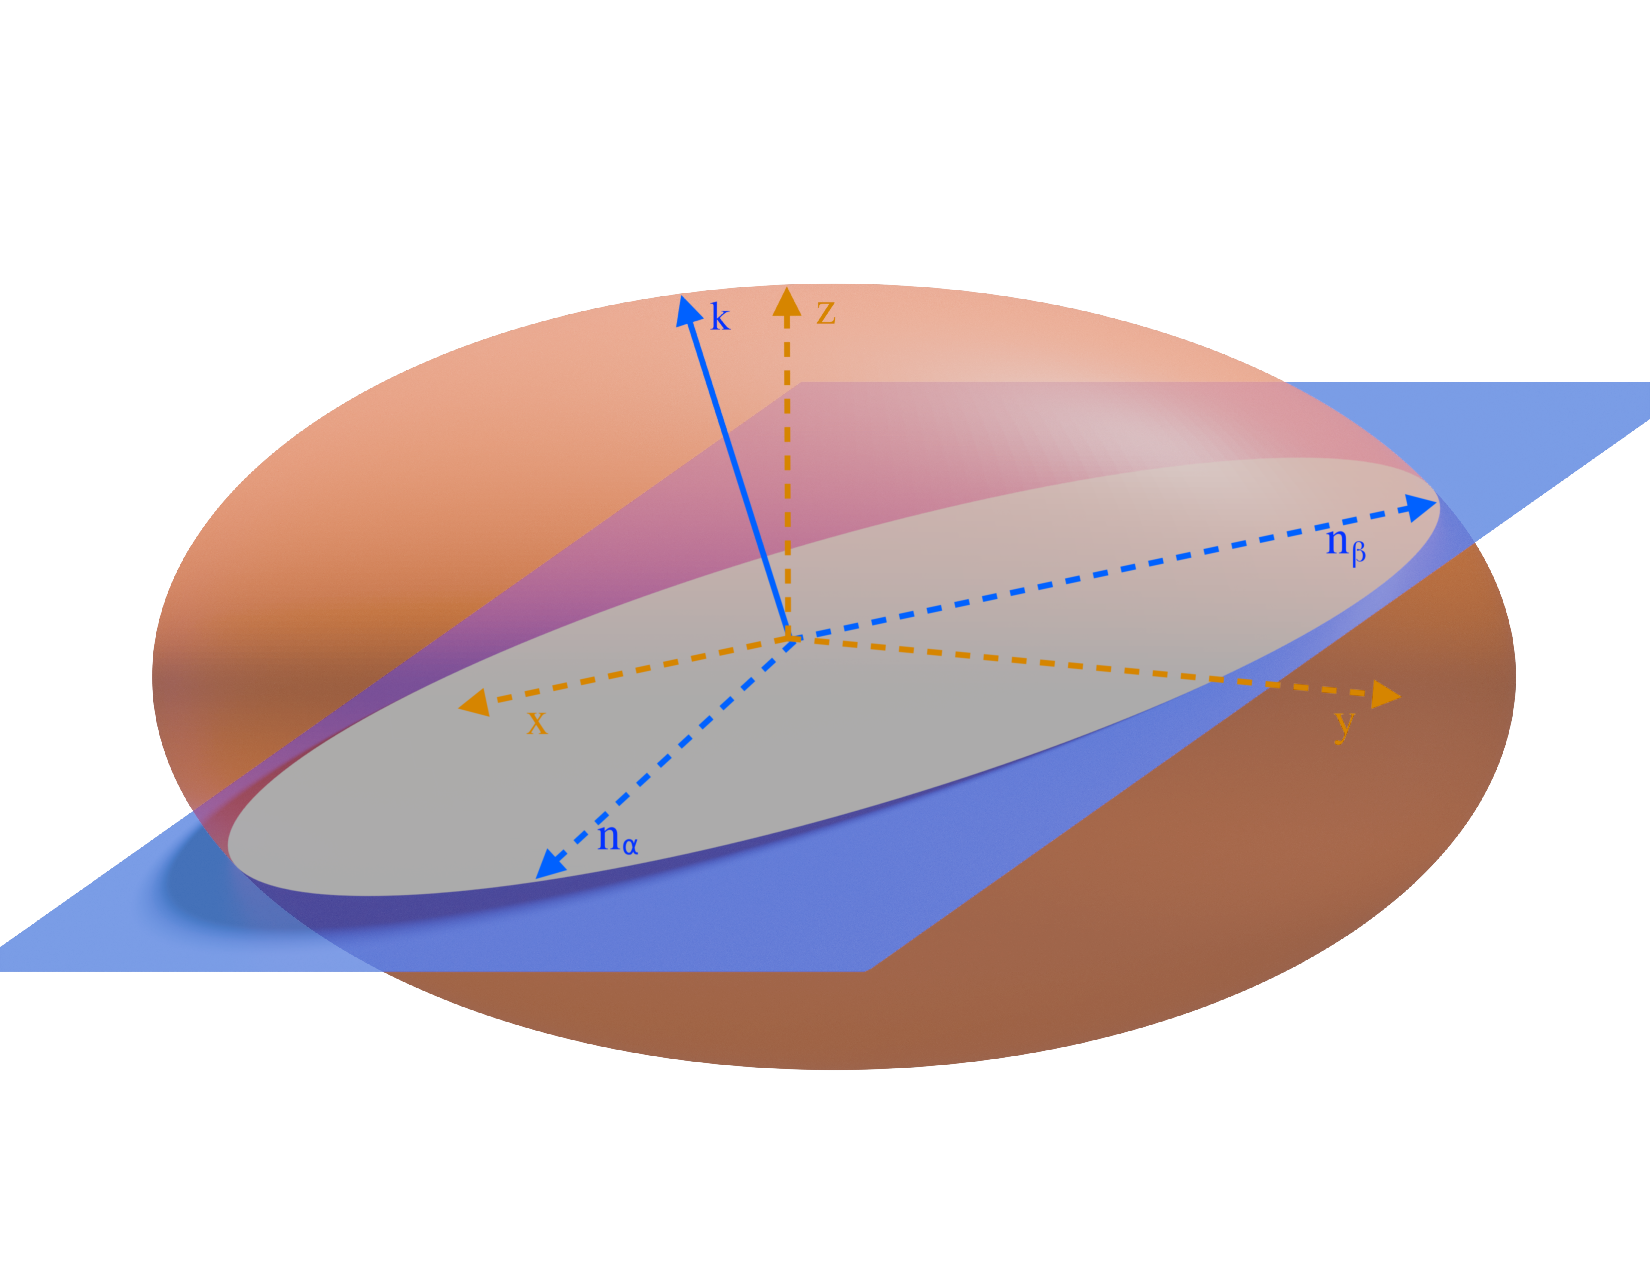
\includegraphics[width=.85\textwidth]{figs/ALGAAS/indicatrix_alph.pdf}
\end{center}
\caption{A surface of uniform energy density ($U_E$) forming an ellipsoid in D-space for a generalized uniaxial crystal with general wavefront propogation indicated by a plane normal $\hat{k'}$ where the major and minor axes of the ellipse cross section indicate slow and fast axes $n_\beta$ and $n_\alpha$ respectively.}
\label{fig:genindtrx}
\end{figure}

The construction begins when considering a constant electric energy density ($U_e$) surface in the $\vec{D}$ space; which forms an ellipsoid: 

\begin{equation}\label{eq:lagr1}
\frac{D_x}{\varepsilon_x} + \frac{D_y}{\varepsilon_y} + \frac{D_z}{\varepsilon_z} = 2 U_e \varepsilon_o
\end{equation}
With redefined coordinates $(\vec{D}/\sqrt{2 U_e \varepsilon_o}) \rightarrow \vec{r}$ and setting $\varepsilon_i = n^2_i$:
\begin{equation}
\frac{x^2}{n_x^2} + \frac{y^2}{n_y^2} + \frac{z^2}{n_z^2} = 1
\end{equation}

This equation for the ellipsoid is known as the indicatrix. Given the co-planar solution demonstrated in the last section, we can impose the normal of the plane $\vec{r} \cdot \vec{s} = 0$:

\begin{equation}\label{eq:lagr2}
\vec{r} \cdot \vec{s} = x s_x + y s_y + z s_z = 0
\end{equation}
\autoref{eq:lagr1} and \autoref{eq:lagr2} both contribute constraints to the method of finding extrema using Lagrange multipliers for the function:
\begin{equation}
r^2 = x^2 + y^2 + z^2
\end{equation}
The Lagrangian ($\mathcal{L}$) with the introduced multiplers ($\lambda_1$, $\lambda_2$) then becomes:
\begin{equation}
\mathcal{L}(\textcolor{red}{\vec{r},\vec{s}},\lambda_1, \lambda_2) =
x^2 + y^2 + z^2 + \lambda_1 (xs_x + ys_y + zs_z) + \lambda_2 \bigg( \frac{x^2}{\varepsilon_x} + \frac{y^2}{\varepsilon_y} + \frac{z^2}{\varepsilon_z} - 1 \bigg)
\end{equation}
With the generated system of equations from the Lagrange multipler method ($\partial F_i/ \partial x_i = 0$, and $\partial F_j/ \partial \lambda_j$) where index $i =x,y,z$ and $j = 1,2$ we obtain a system of 3 equations:
\begin{equation}
i \bigg(1-\frac{r^2}{\varepsilon_{i}} \bigg) + s_{i} \bigg(\frac{x s_x}{\varepsilon_x} + \frac{y s_y}{\varepsilon_y} + \frac{z s_z}{\varepsilon_z} \bigg) = 0
\end{equation}
The result is verified when substituting $r \rightarrow \frac{\vec{D}}{\sqrt{\vec{E} \cdot \vec{D} \varepsilon_o}}$ back which recovers \autoref{eq:modelec}.
\\
\subsection{\texorpdfstring{$\gaas$}{gaas} and \texorpdfstring{$\algaas$}{algaas} crystal classification}
The space group of $\gaas$ as well as $\algaasgen$ are within the $F\bar{4}3m$ space group. Crystals of this space group are commonly known as zincblende crystals; a common crystal configuration named after zinc sulfide (ZnS). Also categorized as a cubic crystal, their crystallographic structure displays linear optical isotropic characteristics when stress free and no DC and/or slowly varying electric fields are present~\cite{boyd:2008}. 

\begin{figure}[!ht]
\begin{center}
\includegraphics[width=.5\textwidth]{figs/ALGAAS/gaas_unit_cell_mi.pdf}
\caption{The unit cell of gallium arsenide (GaAs) with associated miller indices as coordinate axes}
\end{center}
\label{fig:gaasuc}
\end{figure}

Zincblende structures, like the crystalline materials in question can exhibit birefringent properties when under influence of mechanical stresses and static / low-frequency electric fields ($E_\mathrm{STLF}$); characterized by photoelastic and electro-optic effects respectively. Birefringence witnessed from HR $\gaas$ coatings is said to be due to an ``intrinsic stress" in the high and low index layers (Due to heteroepitaxial bonds between them from a noticiable difference in lattice cell constant between $\gaas$ and $\algaas$)~\cite{adachi:1985}.

\subsubsection{Linear electro-optic effect (Pockel's effect)}
For non-centrosymmetric crystalline media there exists a non-zero rank 2, $6 \times 3$ tensor ($r_{ij}$) connecting a low-frequency \footnote{``low frequency'' meaning orders of magnitude smaller than an optical field it effects} electric field $\vec{E}(f) = [E_x(f), E_y(f), E_z(f)]$ directly to the \hyperref[sec:indicatrix]{indicatrix} ~\cite{yariv,nye}:
\begin{equation}
  \left[ {\begin{array}{c}
   \big( \frac{1}{\Delta n ^2 } \big)_1 \\
   \big( \frac{1}{\Delta n ^2 } \big)_2 \\
   \big( \frac{1}{\Delta n ^2 } \big)_3 \\
   \big( \frac{1}{\Delta n ^2 } \big)_4 \\
   \big( \frac{1}{\Delta n ^2 } \big)_5 \\
   \big( \frac{1}{\Delta n ^2 } \big)_6 \\
  \end{array} } \right]
  =
%
 \left[ {\begin{array}{ccc}
   r_{11} & r_{12} & r_{13}\\
   r_{21} & r_{22} & r_{23}\\
   r_{31} & r_{32} & r_{33}\\
   r_{41} & r_{42} & r_{43}\\
   r_{51} & r_{52} & r_{53}\\
   r_{61} & r_{62} & r_{63}\\
  \end{array}} \right]
 %
 \left[{\begin{array}{c}
   E_x (f)\\
   E_y (f)\\
   E_z (f)\\
 \end{array}} \right]
\end{equation}

\noindent The $i$ index runs over the terms in the indicatix equation:
\begin{equation}
\bigg(\frac{1}{\Delta n_x^2} \bigg) x^2\ + \bigg(\frac{1}{\Delta n_y^2} \bigg) y^2 + \bigg(\frac{1}{\Delta n_z^2} \bigg) z^2 + 2 \bigg(\frac{1}{\Delta n_{xz}} \bigg)xz + 2 \bigg(\frac{1}{\Delta n_{yz}} \bigg)yz + 2 \bigg(\frac{1}{\Delta n_{xy}} \bigg)xy = 1
\end{equation}

%%Detail on some prior knowledge of $f \leq f_\mathrm{max}$? (Pockels cell specs?)

\subsubsection{\texorpdfstring{$r_{ij}$}{rij} for zincblende crystals (\texorpdfstring{$r_{\bar{4}3m, ij}$}{r43})}

The form of the electro-optic tensor for zincblende crystals (including $\gaas$ and $\algaas$) reduces such that $r_{ij} = r_{41} = r_{52} = r_{62} \neq 0$ with all other terms being zero:

\begin{equation}
r_{\bar{4}3m,ij} =
 \left[ {\begin{array}{ccc}
  0 & 0 & 0\\
  0 & 0 & 0\\
  0 & 0 & 0\\
  r_{41} & 0 & 0\\
  0 & r_{52} & 0\\
  0 & 0 & r_{63}\\
 \end{array}} \right]
\end{equation}

\noindent Where also $r_{41} = r_{52} = r_{63}$

\subsubsection{New principal (electro-optic) dielectric axis for zincblende structures}
In general the principle dielectric axes of the new ellipsoid do \textbf{not} coincide with the axes of the ellipsoid of the unperturbed crystal. The form of the index ellipsoid for a zincblende crystalline material accounting for the electro-optic tensor and some generalized DC electric field $\vec{E}$ expressed in terms of the crystallographic axes is given by:
\begin{equation}\label{eq:zindicatrix}
\bigg(\frac{1}{n_o^2} \bigg) x^2\ + \bigg(\frac{1}{n_o^2} \bigg) y^2 + \bigg(\frac{1}{n_o^2} \bigg) z^2  + 2r_{41} E_{[100]} yz + 2r_{41} E_{[010]} xz + 2r_{41}E_{[001]} xy= 1
\end{equation}

\noindent Where we have set $n_x = n_y = n_z = n_o$ for zincblende structures.

\noindent Eigenvectors of the above tensor equation, produce the two principal axes:	

\begin{equation}
 \left[ {\begin{array}{ccc}
   \big( \frac{1}{n_o ^2} \big)& r_{41}E_{[001]} & r_{41} E_{[010]}\\
   r_{41}E_{[001]} & \big( \frac{1}{n_o ^2} \big) &  E_{[100]}\\
   r_{41} E_{[010]} & r_{41} E_{[100]} & \big( \frac{1}{n_o ^2} \big)\\
  \end{array}} \right]
\end{equation}

\subsubsection{The photoelastic effect}

General stresses and strains of a material may also cause transformations to the indicatrix through the rank 4 elasto-optical tensor $p_{i j k l}$:

\begin{equation}
 \bigg( \frac{1}{\Delta n^2} \bigg)_{ij} = p_{ijkl} \epsilon_{kl}
\end{equation}

\noindent Where the strain ({\boldmath$\epsilon$}) relates to stress ({\boldmath$\sigma$}) using the generalized Hooke's law: 
%\begin{equation}\label{eq:indicgen_stress2strain}
%	\epsilon_{\alpha \beta} = r_{\gamma \alpha \beta}E_{\alpha} + s_{\alpha \beta \gamma \theta } \sigma_{\gamma \theta}
%\end{equation}
% elasto-optic ($p_{ij \alpha \beta}$) tensor to the stress tensor ($\epsilon_{\alpha \beta}$) via stress-strain / piezoelectric relations:
\begin{equation}\label{eq:genhookeslaw} 
 \begin{split}
	 \epsilon_{ij} = K_{ijkl} \sigma_{kl}
	 \\
	 \sigma_{ij} = C_{ijkl} \epsilon_{kl}
 \end{split}
\end{equation}
And also form a connection between the elasto-optical tensor to the piezo-optical tensor
\begin{equation}\label{eq:indicgenelastooptical}
 \begin{split}
	p_{ijkl} = \pi_{ijkl} C_{klrs}
	\\
	\pi_{ijrs} = p_{ijrs} K_{rskl}
 \end{split}
\end{equation}
For realistic mirror coatings, heteroepitaxial bonding between $\gaas$/$\algaas$ layers may produce an intrinsic strain within the HR stack and can lead to the existence of a static non-negligible birefringence throughout the coating layers \cite{cole:2016}.

\subsubsection{The generalized indicatrix}
Both forms of the induced birefringence (electro-optic and photo-elastic) can be incorportated into a condensed form \cite{nye}:

\begin{equation}\label{eq:indicgen}
	\bigg( \frac{1}{\Delta n^2} \bigg)_{ij} = r_{ijk}E_k + p_{ijkl} \epsilon_{kl}
\end{equation}


%%New principal dielectric axes for zincblende structures (zinblende photoelastic tensor, zincblende electro-optic tensor)

\subsection{EO Modulation}\label{sec:EOM}
Imparting phase modulations onto an optical carrier field is a common application of the electro-optic effect. Electro-optic modulators (EOMs) or Pockel cells are sold as a standard optical components usually composed of a monolithic crystalline material sandwiched between two capacitor plates connected to a single electrical input port (typically coaxial for RF) designed to take in a voltage input of frequency ($\Omega$) within a specified modulation amplitude and frequency bandwidth. When the field amplitude across the crystal is driven by a voltage controlled oscillation, the amplitudes of the electro-optic tensor vary linearly. 

\begin{figure}[H]
    \centering
    \includegraphics[width=.5\textwidth]{figs/ALGAAS/eom_l_assembly.pdf}
    \\
    \vspace{-9mm}
    \includegraphics[width=.5\textwidth]{figs/ALGAAS/eom_t_assembly.pdf}
\caption{Longitudinal and transverse electro-optic modulators}
\label{fig:EOM_types}
\end{figure}

The voltage amplitude of the signal input is proportional to the strength of the modulated phase on the optical carrier frequency ($\omega$); commonly quantified in terms of a modulation index ($\beta$):

%%Consider a specific crystal that gives us our $\beta \mathrm{sin}(\Omega t)$

\begin{equation}\label{eq:inpEOM}
	E_\mathrm{out} = E_o e^{i \omega t + \beta \mathrm{sin}( \Omega t)} \approx E_o [J_o(\beta)e^{i \omega t} + J_1(\beta) e^{i(\omega + \Omega)t} - J_1(\beta) e^{i(\omega - \Omega)t}]  
\end{equation}

\noindent Where we have approximated with the Jacobi-Anger expansion utilizing Besssel functions of the first kind ($J_n(x)$) ~\cite{oliver:1972}:

\begin{equation}\label{eq:jacobianger}
	e^{iz \mathrm{sin}(\theta)} \approx J_0(z) + 2 \sum_{n=1}^{\infty} i^n J_n(z) \mathrm{sin} (n \theta)
\end{equation}

\ref{eq:inpEOM} sufficiently demonstrates that, to the first order, a carrier field that is phase modulated is also, in essence, imparting power to separate optical sideband fields separated in frequency by an integer multiple of the modulation $n \cdot \Omega$. Typically $\Omega$ is a chosen frequency used for optical heterodyne detection; while for a noise-driven modulation, the phase coupling is coorelated to the local directionally relevant E-field spectra alongside the propogation length of the beam propogation within the electro-optic media.

\subsection{Optical anisotropy of a HR \texorpdfstring{$\gaas$}{gaas} / \texorpdfstring{$\algaas$}{algaas} stack}
A comprehensive survey of relevant birefringent properties of a HR $\gaas$/$\algaas$ mirrorstack is due, and for this body of work includes: 1) crystal coordinate considerations when asserting an optical axis on a highly reflective crystalline stack manufactured by the Thorlabs crystalline coatings division, 2) citations of coating parameters and observed intrinsic birefringence from the highly reflective coating stack in question, 3) analysis of the differential electro-optic effect on the phase of a reflected beam, and 4) estimating the the differential phase noise in LIGO based on preliminary electric field measurements measured at LHO.
\subsubsection{Miller indices for highly reflective $\gaas$/$\algaas$ coatings}

\begin{figure}[!hb]
    \begin{subcaptiongroup}
	    \includegraphics[width=.5\textwidth]{figs/ALGAAS/coating_orientation_normal.pdf}
	    \phantomcaption\label{conormal}
	    \includegraphics[width=.5\textwidth]{figs/ALGAAS/coating_orientation_isometric.pdf}
	    \phantomcaption\label{coiso}
    \end{subcaptiongroup}
\caption{The beam propogation axis ($\vec{S}$, $[-100]$) with respect to the $\gaas$/$\algaas$ crystal axes. The axis formed by the [100] plane normal is drawn parallel with the beam axis (z-axis) and the polarizations of incident and reflected beam oscillate along vectors within the plane formed by the normal of that axis. The coating is grown with a flat tracing a line within the [0-11] plane; where the plane normal points towards the sample center.}
\label{fig:algaascoords}
\end{figure}

Up to this point three varieties of orthonormal coordinates are addressed: the crystal axis (as indicated by Miller index plane normals), the principal dielectric axis (based on diagonalization of the indicatrix), and an optical beam axis (when considering a desired (laser) light propogation). The asserted beam axis can be cited \autoref{fig:algaascoords}.

\subsubsection{Electro-optic coupling to the reflected phase of a HR mirror coating}
With our chosen beam axis, the influence of an isotropic white noise field ($E_N = [E_{Nx},E_{Ny},E_{Nz}]$) is considered:

\begin{equation}
 \left[ {\begin{array}{ccc}
   \big( \frac{1}{n_o ^2} \big)& r_{41}E_{Ny} & r_{41} E_{Nx}\\
   r_{41}E_{Ny} & \big( \frac{1}{n_o ^2} \big) & r_{41} E_{Nz}\\
   r_{41} E_{Nx} & r_{41} E_{Ny} & \big( \frac{1}{n_o ^2} \big)\\
  \end{array}} \right]
\end{equation}

\noindent Assuming $E_N$ is small, the indicatrix change of $E_{Nx}$ and $E_{Ny}$ relative to $E_{Nz}$ (as seen by the beam polarization) will be small ($r_{41}E_{N(x/y)} \ll r_{41}E_{Nz}$). After diagonalizing with relevant terms \footnote{Note that the form of the tensor is still in the crystal coordinates but the $E_n$ terms are placed in the tensor such that their directions align with beam axis coordinates.} in the tensor, we are left with the following eigenindices:

\begin{equation}
\begin{aligned}
n_x' & = n_o - r_{41}E_{Nz} \\
n_y' & = n_o + r_{41}E_{Nz}
\end{aligned}
\end{equation}

%How the modulation of the phase of the carrier field is dependent on the orientation of its wave vector with respect to the crystal structure, the modulating electric field direction and strength, (other items to discuss in terms of introducing the effect)
%% For GaAs @ $10.6\mu$ $r_{41} = 1.6 \times 10^{-12}$ [m/V]
%% Adachi estimate for $\mathrm{Al_{x}Ga_{1-x}As}$?
%% Relevant eigenpolarizations, non-optical field $E_y = E_z = 0$?}
%% FIGURE: SUB1 Transformed indicatrix (Before and after $E_x$)
%% FIGURE: SUB2 Ellipse cross section. New eigenpolarizations and corresponding indices and their influence on incident field (Marty's result)

\noindent Assuming we are operating in a coordinate system suggested in \autoref{fig:algaascoords}, which plane is impacted by some $E_\mathrm{noise}$? Revisiting the \autoref{eq:zindicatrix} we can see that for even non-zero z and y components that the only coupling to the input beam polarization is the index along the cross coupled zy-axis through $E_z$ is that of the $E_x$ term. This gives us the ability to easily diagonalize the indicatrix tensor when setting non-relevant field terms to zero.
\\
Fejer and Bonilla take an analytical approximation approach when finding the impact of the electric field to the change in phase of the light through a crystalline anisotropic thin film ($\lambda/4$) stack \cite{bonillafejer}.

\begin{equation}
\hat{\phi}' = \frac{\pi n_1 z}{1-z^2}(z^{2N} -1) \frac{z^{2N} \frac{(n_f)^2}{n_2 n_3}(n_2 \kappa_{\gamma 2} + n_3\kappa_{\gamma 3}) - (n_2 \kappa_{\gamma 3} + n_3\kappa_{\gamma 3})}{(n_1)^2 -(n_f)^2 z^{4N}}
\end{equation}

with $z = \frac{n_2}{n_3}$
and
$
\kappa_{\gamma j} = \frac{d}{d \gamma} \mathrm{log}(n_j h_j)|_{\gamma =\gamma_{O}} \bigg(\frac{\hat{n}_j'}{\hat{n}_j} +\frac{\hat{h}_j'}{\hat{h}_j} \bigg)
$

With $\kappa$ being a scalar parameter.
%%FIGURE: Cross sectional view of multilayer coating

\begin{figure}[!ht]
	\includegraphics[width=\textwidth]{figs/ALGAAS/ALGAAS_HR_layers_ann.pdf}
\caption{The beam propogation axis ($\vec{S}$, $[-100]$) with respect to the $\gaas$/$\algaas$ crystal axes. The axis formed by the [100] plane normal is drawn parallel with the beam axis (z-axis) and the polarizations of incident and reflected beam oscillate along vectors within the plane formed by the normal of that axis. The coating is grown with a flat indicating a line within the [0-11] plane; where the plane normal points towards the sample center.}
\label{fig:HRlayers}
\end{figure}


\subsubsection{Numerical estimate}

In the appendix of \cite{ballmer:2015} Ballmer constructs a coating layer transfer function for a given coating layer k with index $n_k$, and thickness $d_k$, defining right and left propogating modes $\psi^{R,L}$ repsectively:
$$
  \left[ {\begin{array}{c}
   \psi^\mathrm{R} \\
   \psi^\mathrm{L} \\
  \end{array} } \right]_{k+1}
  =
%
Q_k D_k
%
 \left[{\begin{array}{c}
   \psi^\mathrm{R} \\
   \psi^\mathrm{L} \\
 \end{array}} \right]
$$
\noindent $D_k$ applies the phase ($\phi_k = 4\pi n_k d_k /\lambda_0$) from a given coating layer, and $Q_k$ applies the transfer function between high-low/low-high index layers transition:

\begin{equation}
D_k =
\left[ {\begin{array}{cc}
  e^{-i \phi_k / 2}& 0\\
 0 & e^{i \phi_k / 2}\\
\end{array} } \right]
\end{equation}

\begin{equation}
Q_k = \frac{1}{2n_{k+1}}
\left[ {\begin{array}{cc}
  n_{k+1} + n_k & n_{k+1} - n_k\\
 n_{k+1} - n_k & n_{k+1} + n_k\\
\end{array} } \right]
\end{equation}
\noindent Defining a HR coating stack, the total transfer matrix from vaccum $Q_0$ to the $N$th coating layer is:
\begin{equation}
	M = Q_N D_N ...Q_k D_k...Q_1D_1Q_0
\end{equation}
\noindent And the partial derivative at the kth coating layer is:

\begin{equation}
	\label{eq:partialM}
	\frac{\partial M}{\partial \phi_k} = Q_N D_N ...Q_{k} \begin{bmatrix} e^{-i \phi_k /2} & 0 \\ 0 & e^{i \phi_k/2} \end{bmatrix} \begin{bmatrix} -i /2 & 0 \\ 0 & i/2 \end{bmatrix} Q_{k-1} D_{k-1}...Q_1D_1Q_0
\end{equation}

\noindent The above representing a collective differential phase manifesting as a sum of these phase components. This explicit perturbed phase at the kth layer for the electro-optic effect ($\partial n_k/\partial E$) is found when:
\begin{equation}\label{eq:EOphasekdiff}
	\frac{\partial \phi_k}{\partial E} = \frac{4 \pi d_k}{\lambda} \frac{\partial n_k}{\partial E} = \pm \frac{ 2 \pi}{\lambda} n_k^3 d_k r_{41,k}
\end{equation}
\noindent Where the electro-optic coefficients $r_{41}$ for $\gaas$ and $\algaasgen$ \cite{suzuki:1984, adachi:2012, adachi:1985}:
\begin{equation}
\begin{aligned}
	& r_{41, \gaas} =  -1.33 \times 10^{-12} & [\mathrm{m} / \mathrm{V}]
	\\ 
	& r_{41, \algaasgen}  = - (1.33 - 0.45x) \times 10^{-12} &  [\mathrm{m}/\mathrm{V}]
\end{aligned}
\end{equation}
\noindent Rather than tagging on the phases individually, an easier computation is found when relying on the relationship between the transmission ($t$) and reflectivity ($r$) to a general transfer matrix (in our case $M$):
$$
	\begin{bmatrix} 1 \\ r \end{bmatrix} \begin{bmatrix} M_{11} & M_{12} \\ M_{21} & M_{22} \end{bmatrix} = \begin{bmatrix} t \\ 0\end{bmatrix}
$$
\noindent And using this relation, differentiating the reflectivity with respect to $\phi_k$:
$$
	\frac{\partial r}{\partial \phi_k} = - \bigg( \frac{1}{M_{21}} \frac{\partial M_{21}}{\partial \phi_k} - \frac{1}{M_{22}}\frac{\partial M_{22}}{\partial \phi_k} \bigg) \frac{M_{21}}{M_{22}}
$$
\noindent The differential reflectivity is normalized by the total reflectivity and taking the imaginary component as noted in~\autoref{eq:partialM}: 

\begin{equation}
	\frac{\partial \phi_c}{\partial \phi_k}  = \mathrm{Im} \bigg(\frac{1}{r} \frac{\partial r}{\partial \phi_k} \bigg) =  \bigg( \frac{1}{M_{21}} \frac{\partial M_{21}}{\partial \phi_k} - \frac{1}{M_{22}}\frac{\partial M_{22}}{\partial \phi_k} \bigg) 
\end{equation}

\noindent The impact of a differential electric noise field ($E_\mathrm{STLF}$) on $M$ due to the electro-optic effect on the kth layer, we use the chain rule:

\begin{equation}
	\bigg| \frac{\partial \phi_c}{\partial  E_\mathrm{STLF}} \bigg| =  \bigg| \frac{\partial \phi_c}{\partial \phi_k}  \frac{\partial \phi_k}{\partial E} \bigg|
\end{equation}

The coating to be studied consists of 36 $\lambda$/4  thick layers of $\gaas$ interspersed with 35 layers of $\lambda$/4 thick $\algaas$. $\gaas$ forms the top and bottom layer to prevent oxygen absorption from the AlGaAs layer. The $\gaas$ layers have an index of $n_{\gaas} = 3.480$ and a thickness of $\Delta d_{\gaas} = 76.43$ nm while the low index $\algaas$ layers are $n_{\algaas} = 2.977$ with thickness $\Delta d_{\algaas} = 89.35$ nm. With the constructed matrices, we apply these parameters and compute a differential phase of:

\begin{equation}
	\bigg| \frac{\partial \phi_c}{\partial  E_\mathrm{STLF}} \bigg|  = 3.9 \times 10^{-11}\; [\mathrm{rad}/\mathrm{V}/\mathrm{m}]      
\end{equation}

%High Index:  GaAs, n=3.480, layer thickness is 76.43 nm
%Low Index:  $ \mathrm{Al}_{0.92} \mathrm{Ga}_{0.08} \mathrm{As} $, n=2.977, layer thickness is 89.35 nm
%Info from Steve. Written source

\subsection{Measured birefringence from HR \texorpdfstring{$\gaas$}{gaas}/\texorpdfstring{$\algaas$}{algaas} mirrors}

There are different accounts of a measured birefringence from HR $\gaas$ / $\algaas$ coatings (\href{https://dcc.ligo.org/DocDB/0181/G2200386/001/G2200386.pdf}{Satoshi}, \href{https://nodus.ligo.caltech.edu:8081/CTN/1474}{CTN}, \href{https://dcc.ligo.org/DocDB/0181/G2200559/001/G2200559-v1\%20-\%20polarization.pdf}{Aidan})

%%Is the measured birefringence static? (Layer bonding method might introduce something?)
%% Does it change from different mounting methods? (Photoelastic) (order of magnitude estimate)
%% Electro-optic ruled out based on field measurements and relative coupling factor.
%% Measurement precision of the coating birefringence? Cavity length, Polarization drifts, etc.
From coating manufacturers it's estimated that static birefringence can arise from the intrinsic strain between hetero-epitaxial layers of $\gaas$/$\algaas$. \cite{cole:2013, adachi:1985}
%% Marty's document about Birefringence in Crystalline mirror coatings V.8

\subsection{Initial projected DARM coupling}
Measured field spectra acquired from installed electric field meters located within LHO and LLO ETMX and ETMY vacuum chambers can help translate how much DARM coupling can occur from electro-optic coating noise. For O3 the EFMs were located next to the test mass mirrors and measured a consistent 3 $[\mu \mathrm{V} / \mathrm{m} / \sqrt{\mathrm{Hz}}]$ @ 100 Hz~\cite{buikema:2020}. This along with computed estimate allows us to create an upper limit for what this noise might be assuming incoherent fields between the end stations and a flat frequency response within LIGO's bandwidth.

% Taking the upper and the lower EFM measurements from ~\cite{efmlog} $.3\; [\mathrm{V}/\mathrm{m}/\sqrt{\mathrm{Hz}]}$ @ 60 Hz and $4\times10^{-3}\; [\mathrm{V}/\mathrm{m}/\sqrt{\mathrm{Hz}]}$ @ 4kHz.
%% \satoshi{I don't think these values are calibrated. According to Martynov et al. 2016, the fluctuations in the electric filed is $\sim10^{-5}\,\mathrm{[(V/m)/\sqrt{Hz}]}$.}

\section{Electro-optic measurement apparatus}
In seeking a calibrated estimate of the electro-optic effect for the $\gaas$/$\algaas$ mirror coating stack, we sought to drive an electro-optic response of a mirror sample from Thorlab's crystalline mirror coatings division placed within a custom longitudinal Pockels cell mirror mount. The assembly, with the installed sample, assumed the end mirror position within a two mirror Fabry-Perot cavity, while resonance of a circulating Nd:YAG 1064nm carrier beam was held by a Pound-Drever-Hall servo. As seen in the prior section, the size of the imparted phase noise for currently existing gravitational wave detector configurations is estimated to be small but notable. Investigation through measurement of said effect requires detection methods with sufficient sensitivity for the differential phase noise imparted by the effect. Details and specifications of the detection schema are discussed along with relevant measurements and results. 

%% Driven acoustic modes of the longitudinal pockels cell mirror mounts lead to numerous mounting strategies that will be detailed below. 


\begin{figure}[H]
	\includegraphics[width=\textwidth]{figs/ALGAAS/algaas_pockels_effect_measurement_schematic.pdf}
	\caption{A simplified and modular schematic of the PDH servo used along with an electrostatic drive mount design comprised of a disk capacitor sandwiching the HR AlGaAs sample, a high voltage amplifier, and a signal / network analyzer.}
\label{fig:simpschema}
\end{figure}
 Measurability of the electro-optic effect is contingent upon two initial design criteria: the sensitivity of the optical plant to be implemented in the PDH servo, and the maximum achievable electric field strength along the beam axis ($|E_z|_\mathrm{max}$).

\subsection{PDH servo}\label{subsubsec:pdh}
The Pound-Drever-Hall technique, originally and commonly used for laser frequency stabilization to an ultra-stable length reference, allows the tracking of the linear phase response of an input carrier field through cavity resonance. The servo fully realizes the ability of an optical cavity to act as a length / frequency discriminator:

\begin{equation}\label{eq:cavlf}
	\frac{\Delta f}{f} = \frac{\Delta L}{L}
\end{equation}

\noindent The alternative side-of-fringe lock provides a linear response in intensity, which is adequate for some applications but with reduced sensitivity due to the required power reduction by operating off resonance. Measurements of phase are extracted through an optical heterodyne; the co-propogation of a separate (but phase-locked) optical field with a known frequency separation to the carrier reflected from the cavity input. The PDH servo bypasses the need for a complicated phase-locked two laser configuration by imposing a phase modulation onto the carrier field via an electro-optic modulator (aka Pockels cell) mentioned in section \autoref{sec:EOM}. Setting a photodiode of area ($A_\mathrm{PD}$) in reflection of the cavity with a coefficient of $r_\mathrm{cav}(\omega,L)$, we measure the reflected power of the input field given by \autoref{eq:inpEOM}\;:

%If the modulation depth given by \ref{eq:inpEOM} is set such that $\beta < 1$ then the input field may be approximated in terms of the first two Bessel functions $J_0$, $J_1$:

%\begin{equation} \label{eq:EOM_trans_field}
%E_\mathrm{inp} \approx E_0 [J_0(\beta)e^{i \omega t} + J_1(\beta)e^{i (\omega + \Omega) t} - J_1(\beta)e^{i(\omega -\Omega)t}]
%\end{equation}
%
%With a high enough modulation frequency the terms given above can be far enough from the carrier frequency, so that the phase modulation onto the carrier field is mathematically and physically equivalent to imposing separate optical fields (sidebands) which in most cases do not resonate in the optical cavity of interest. 



\begin{equation}
 \begin{alignedat}{3}
    &P_\mathrm{refl} && \approx \frac{|E_\mathrm{refl}|^2}{A_\mathrm{PD}} && \\
    & &&\approx \frac{E_0^2}{A_\mathrm{PD}} && \bigg\{J_0^2 |r_\mathrm{cav}(\omega,L)|^2 + J_1^2(\beta)|r_\mathrm{cav}(\omega+\Omega,L)|^2 - J_1^2(\beta)|r_\mathrm{cav}(\omega-\Omega,L)|^2 +  \\
    & && && J_0J_1(\beta)\big[r_\mathrm{cav}\omega,L) r_\mathrm{cav}^*(\omega+\Omega,L)\big] - J_ 0J_1(\beta)\big[r_\mathrm{cav}(\omega,L)r_\mathrm{cav}^*(\omega-\Omega,L)\big]\bigg\}
  \end{alignedat}
\end{equation}

The two trailing terms in the above equation for $P_\mathrm{refl}$ generate a beat frequency term between the carrier and lower and upper sidebands. The magnitude and sign of these beat terms directly relate to the phase of the reflected carrier field and can be measured and transformed to the error signal seen in \autoref{fig:pdherr} using resonant electronics (tuned to a chosen sideband frequency) for amplification and a mixer for demodulation.

\begin{figure}[H]
	\includegraphics[width=\textwidth]{figs/ALGAAS/pdh_error.pdf}
	\caption{By imposing 25 MHz RF sidebands, a pair of reflected reference fields near carrier resonance are off cavity resonance while beating with the carrier and provide a linear response after demodulating the sideband power. With the introduction of high and low frequency sideband fields, their presence is also detected through the DCPDs and PDH error signal. Their separations from carrier resonance are equal in phase (length, and frequency).}
\label{fig:pdherr}
\end{figure}

With this linearity and sensitivity at cavity resonance, implementation into PID feedback is the next task as any small detuning of the cavity can be registered as a drift from the loop's zero point and fed back to an actuator with an estimated calibration gain factor. When implemented into a low-noise design, this servo can also be used for a high sensitivity lock-in measurement; and with well characterized instrumentation, calibration of the induced differential phase of the light within the stable reference cavity into differential length (or frequency).


\subsection{Servo Parameters}
The quantity we are attempting to measure is on the order of a length change of $3.3 \times 10^{-18}$ [m/(V/m)], motivating a short cavity design as the relative differential length (phase) change scales with the sensitivity \autoref{eq:cavlf}. Considerations of the lab mirror inventory and mode matching critera lead us to two candidate plano-concave (ROC = 0.333m) HR IBS coated sample input couplers; one from CVI Melles-Griot and another from ATFilms. When paired with the plano-plano $\gaas$/$\algaas$  mirror from the Crystalline Mirror Solutions (CMS) division of Thorlabs we create a 0.1665 m long cavity.

%\begin{figure}[H]
%\begin{center}
%\includegraphics[width=.80\textwidth]{ALGAAS/opt_layout_b.pdf}
%\end{center}
%\caption{\textcolor{red}{Final figure still pending} Detailed optical schema of the experiment. Components highlighted in magenta indicate laser back-reflection protection and output power control. All optics highlighted in PURPLE indicate their function as alignment and mode matching for locking to a triangular ALIGO PMC \textbf{Multiple citations (DCC doc / Fabian's experiment / Erik's experiment)}. Optics highlighted in YELLOW indicate function for alignment and mode matching to the experimental cavity utilizing the HR $\gaas$/$\algaas$ coated mirror sample. Beam profiling to the sample cavity is indicated. For the sake of the numerous mounting strategies tried, the longitudinal pockels cell mirror mount is kept general with the pictured mirror between two disk capacitors}
%\label{fig:expoptical_layout}
%\end{figure}
%%FIGURE: Servo diagram
%%CAPTION: A simplified diagram of the servo used. The highlighted regions of the schematic are intended to provide a modular view; highlighting the components required for the PDH servo to operate.}

The implemented servo design uses a light source from a Mephisto 2000 NE Nd:YAG (1064nm) laser with a 25 MHz phase modulation from a New Focus Model 4003 IR resonant phase modulator. As indicated in the figure above, the electronics chain can be decomposed into various filter components: $S(f)$, $A(f)$, and $A_\mathrm{thermal}(f)$

\subsubsection{Sensing S(f)}
The sensing filter electronics are composed of a single element photodiode (from?) with a QE of ? and the response found in appendix ?. The signal is then mixed with a 25 MHz oscillator phased 180 degrees ? m of cable so the measured beat signal while sweeping through resonance generates the PDH error signal profile \footnote{\autoref{fig:pdherr}}.
\begin{itemize}
\item 25 MHz RFPD
\begin{itemize}
\item Transimpedance measurement (necessary? or should I just use the mixer out PDH to summarize PD/mixer response)
\end{itemize}
\item Frequency Stabilization servo (modified MIT FSS (DCCD980536)) (LTspice model in appendix)
\end{itemize}


\subsubsection{Actuation A(f)}
\begin{itemize}
\item Mephisto 2220 PZT response (capacitance estimated from HVA drive measurement with and without connection to PZT)
\item Channel 3 of SVR 350-3 BIP High Voltage Amplifier from Piezomechanik GmbH with Pomona box (elog 412)
%%FIGURE: Frequency response of A(f)}

\end{itemize}

\subsubsection{Low frequency servo (Thermal loop)}
\begin{itemize}
\item Passed signal from FSS $\rightarrow$ integrators $\rightarrow$ Laser thermal actuator input
\end{itemize}

\subsubsection{OLG(f)}
Isn't quite $\mathrm{A}(f)*\mathrm{S}(f)$ as stated. Doesn't entirely account for the optical plant.
How the measurement is taken (important to take between installations to account for the changes in the optical plant) (elog 831)

\begin{figure}[H]
\begin{center}
\includegraphics[width=\textwidth]{ALGAAS/olg_compare.pdf}
\end{center}
\caption{Comparison of the open loop gain measurement against the multiplied servo electronics measurements. The maximum gain difference is about a factor of 2.8 which is low passed to a difference of 2.0.}
\label{fig:OLGcompare}
\end{figure}

\subsection{Longitudinal Pockels Cell mirror mount assembly}
Maximizing a controlled and well defined electric field ($|E_z|$) within the coating while requiring a through beam to and through the HR coating lead us to a design very similar to that of a longitudinal pockels cell. The most common assembly in for this study is comprised of two electrodes with a 3mm central aperture which is chosen to be at least 5 times larger than the beam size at the plate locations; to avoid significant beam clipping while maximizing field strength at the coating region of interest. There is also a required separation of at least 1/4" accounting for the thickness of the optical sample. Considering these constraints, modelling the system and computing the estimated field strength screened by the coating is the next step to the construction of the assembly.

\begin{figure}[H]
\begin{center}
\includegraphics[width=\textwidth]{ALGAAS/longitudinal_pockels_cell_raw_isometric.pdf}
\end{center}
\caption{Concept image of the longitudinal Pockels cell assembly}
\label{fig:pckcellconcept}
\end{figure}

\subsubsection{Modeling}
The field screened by the coating can be computed from Gauss' Law:
\begin{equation}
\nabla \cdot D = \rho_\mathrm{free}
\end{equation}

\noindent There is no free charge within the region of interest ($\rho_\mathrm{free}=0$), though the optic sample fused silica substrate with the AlGaAs coating imposes dielectric material between the plates. Boundary conditions are expressed in terms of the differential plate potential $V$, so it is natural to first solve the potential ($V$) for all relevant system coordinate points.  


\paragraph*{Boundary Conditions}

\begin{figure}[H]
  \centering
  \includegraphics[width=\textwidth]{ALGAAS/longitudinal_pockels_cell_bc.pdf}
  \caption{Side view of the longitudinal pockels cell mount. The figure is annotated with relevant parameters to build the numerical model}
  %%Use relevant cross sectional figure to establish coordinates for $\gaas$/$\algaas$, as well as the fused silica substrate so the computation is transparent.} Cross sectional diagram indicating relevant axes and boundary conditions utilized in the numerical computation
  \label{fig:laplacecoords}
\end{figure}

\begin{equation}\label{eq:cyllap}
\nabla^2 V = 0
\end{equation}

\subparagraph*{Substrate:}
$ -t_{opt} \; \textless \; z \; \textless \;\mathrm{t}_{opt} $ and $\mathrm{r} \; \textless \;\mathrm{r}_{opt}$
\subparagraph*{Coating}
$\mathrm{t}_{opt} \; \textless \; z \; \textless \;\mathrm{t}_{opt} +\mathrm{t}_{coat} $ and $\mathrm{r} \; \textless \;\mathrm{r}_{opt} $

\subparagraph*{Driven Electrode (V):}
$\mathrm{t}_{cap} \; \textless \; z \; \textless \;\mathrm{t}_{cap} + 2t_{el} $ and $\mathrm{r}_{ap} \; \textless \;\mathrm{r} \; \textless \;\mathrm{r}_{d} $

\subparagraph*{Grounded Electrode (GND):}
$ -t_{cap} -2t_{el} \; \textless \; z \; \textless \; -t_{cap} $ and $\mathrm{r}_{ap} \; \textless \;\mathrm{r} \; \textless \;\mathrm{r}_{d} $

\paragraph*{Numerical Recipe (Finite Differencing)}

We exploit the chosen optic / disk symmetry about the polar angle ($\partial V / \partial \theta = 0$) and compute for the longitudinal ($z$) and radial ($r$) coordinates with the use of the appropriate Laplacian:

\begin{equation} 
\bigg[\frac{1}{r}\frac{\partial}{\partial r} \bigg( r \frac{\partial}{\partial r}\bigg) + \frac{\partial^2}{\partial z^2} \bigg](\varepsilon V) = 0
\end{equation}

Where $\varepsilon$ is the dielectric

Observing equation \autoref{eq:cyllap} we parse the non-zero expression into it's individual parts:

\begin{equation} \label{eq:cyllap_xpand}
    \bigg[\underbrace{\frac{\partial^2}{\partial z^2}}_\text{(c)} + \underbrace{\frac{\partial^2}{\partial r^2}}_\text{(b)}  + \underbrace{\frac{1}{r} \frac{\partial}{\partial r}}_\text{(a)}\bigg] (\varepsilon V) = 0
\end{equation}

\subparagraph*{Term (a)}

Starting with the first derivative, we use the central difference approximation:

\begin{equation}
    \frac{\partial}{\partial r} \rightarrow \frac{f(r + h, z) - f(r - h, z )}{2h} \rightarrow \bigg[-\frac{1}{2} \quad  0  \quad \frac{1}{2} \bigg]
\end{equation}

\subparagraph*{Term (b)}

Second derivative approximation, we use the standard 2d laplace stencil

\begin{equation}
    \frac{\partial}{\partial r^2} \rightarrow \frac{f(r+h, z) - 2 f(r, z) + f(r-h, z)}{h^2} \rightarrow \big[ 1 \quad -2 \quad 1 \big]
\end{equation}

\subparagraph*{Term (c)}
Equivalent to the second derivative approximation used above:

\begin{equation}
    \frac{\partial}{\partial z^2} \rightarrow  \frac{f(r, z+h) - 2 f(r, z) + f(r, z-h)}{h^2} \rightarrow \big[ 1\quad -2 \quad 1 \big]
\end{equation}

To build the stencil terms at the boundaries, we look at the specialized finite difference condition @ $ r = 0 $, with the symmetry about $r=0$ allowing to set ghost point V(-h,z) as V(h,z) :

\begin{equation}\label{eq:first_deriv_V}
	\frac{\partial V}{\partial r} = 0 \rightarrow V(h, z) = V(-h,z)
\end{equation}

\begin{equation}\label{eq:second_deriv_V}
	\frac{\partial^2 V}{\partial r^2} = \frac{2}{h}\bigg(\frac{V(h,z) -  V(0, z) }{h}\bigg) 
\end{equation}

\autoref{eq:first_deriv_V} alone does not define V(0,z), to establish the form of this point, we proceed to (Taylor) expand the function about it:

\begin{equation}\label{eq:taylor_V}
 V \approx V_0  + C_1 r +  C_2 r^{2} + \mathcal{O}(r^4) 
\end{equation}

Symmetry about the origin imposes an even function of $V$:  
$$ \frac{\partial V}{\partial r} \approx C_1 +  2 C_2 r  + \mathcal{O}(r^3) $$

\begin{equation}\label{eq:taylor_terma}
	\frac{1}{r} \frac{\partial V}{\partial r} \approx  2 C_2  + \mathcal{O}(r^2)
\end{equation}

Where $C_1 = 0$ to avoid a singular point.

\begin{equation}\label{eq:taylor_termb}
	\frac{\partial^2 V}{\partial r^2} \approx 2 C_2 + \mathcal{O}(r^2) 
\end{equation}

Substituting \autoref{eq:taylor_terma} and \autoref{eq:taylor_termb} back into equation \autoref{eq:cyllap_xpand} :
\begin{equation}
    \nabla^2 (\varepsilon V)= \frac{\partial^2}{\partial z^2} + 4 C_2 
\end{equation}

The radial portion of the operator $\nabla^2 V$ given \autoref{eq:taylor_V} and \autoref{eq:second_deriv_V}:

\begin{equation}
\bigg(\frac{r_0}{h} - \frac{2}{h^2} \bigg) C_1 + \bigg(\frac{r_h}{h} + \frac{2}{h^2} \bigg) C_2 h^2 = 4 C_2
\end{equation}

Where again, we found $C_1 = 0$:

$$
(r_h * h + 2) C_2 = 4 C_2
$$

\begin{equation}
	r_h = 2 / h
\end{equation}

\begin{equation}
	r_0 = -2 / h
\end{equation}

\newpage
Now meshgrid coordinates are set:

\input{notes/LaplacE_operators.tex}

\newpage

Parallel computation of the potential over the entire meshgrid is done by vectorizing the potential:

\[ 
 \begin{aligned}
    V &= \begin{bmatrix}
           V(\rho_0, z_0) \\
           V(\rho_1, z_0) \\
           \vdots \\
	   V(\rho_n, z_0) \\
	   ---------- \\
	   V(\rho_0, z_1) \\
           V(\rho_1, z_1) \\
           \vdots \\
	   V(\rho_n, z_1) \\
	   ---------- \\
	   \vdots \\
	   ---------- \\
	   V(\rho_0, z_{n-1}) \\
           V(\rho_1, z_{n-1}) \\
           \vdots \\
           V(\rho_n, z_{n-1}) \\
           ---------- \\
           V(\rho_0, z_n) \\
	   V(\rho_1, z_n) \\
	   \vdots \\
	   V(\rho_n, z_n) 
         \end{bmatrix}
  \end{aligned}
\]

\newpage
\noindent Inspired by the second-order elliptic equation, operators are modified to incorporate the following boundary conditions~\cite{Press:2007}:

\[ 
\mathcal{L}_{cyl} = 
\begin{bmatrix} \,
O_{n} & O_{n} & O_{n} & O_{n} & O_{n} & \cdots & \cdots & \cdots & \cdots & \cdots & O_{n}\\
\mathcal{I}_{n} & \mathcal{K}_{n}^{*} & \mathcal{I}_{n} & O_{n} & O_{n} & O_{n} & O_{n} & O_{n} & O_{n} & O_{n} & \vdots\\
O_{n} & \mathcal{I}_{n} & \mathcal{K}_{n}^{*} & \mathcal{I}_{n} & O_{n} & O_{n} & O_{n} & O_{n} & O_{n} & O_{n} & \vdots\\
O_{n} & O_{n}  & \mathcal{I}_{n} & \mathcal{K}_{n}^{*} & \mathcal{I}_{n} & O_{n} & O_{n} & O_{n} & O_{n} & O_{n} & \vdots\\
\vdots & O_{n}  & O_{n}  & \ddots & \ddots & \ddots & O_{n} & O_{n} & O_{n} & O_{n}  & \vdots \\
\vdots & O_{n}  & O_{n}  & O_{n}  & \ddots & \ddots & \ddots & O_{n} & O_{n} & O_{n} & \vdots \\
\vdots & O_{n}  & O_{n}  & O_{n} & O_{n} & \ddots & \ddots & \ddots & O_{n} & O_{n}  & \vdots \\
\vdots & O_{n}  & O_{n}  & O_{n} & O_{n} & O_{n} & \mathcal{I}_{n} & \mathcal{K}_{n}^{*} & \mathcal{I}_{n} & O_{n}  & \vdots\\
\vdots & O_{n}  & O_{n}  & O_{n} & O_{n} & O_{n} & O_{n} & \mathcal{I}_{n} & \mathcal{K}_{n}^{*}  & \mathcal{I}_{n} & O_{n}\\
\vdots & O_{n} & O_{n} & O_{n} & O_{n} & O_{n} & O_{n} & O_{n} & \mathcal{I}_{n} & \mathcal{K}_{n}^{*} & \mathcal{I}_{n}\\
O_{n}      & \cdots & \cdots & \cdots & \cdots & \cdots & O_{n} & O_{n} & O_{n} & O_{n} & {O}_{n}
\end{bmatrix} 
\]

\[
    \mathcal{K}_n^{(1)} = 
\frac{1}{h}
\begin{bmatrix*}[c] \,
0 & 0 & 0 & 0& 0 & \cdots & \cdots & \cdots & \cdots & \cdots & 0 \\
\frac{1}{2} & 0 & \frac{1}{2} & 0 & 0 & 0 & 0 & 0 & 0 & 0 & \vdots \\
0 & \frac{1}{4} & 0 & \frac{1}{4} & 0 & 0 & 0 & 0 & 0 & 0 & \vdots \\
0 & 0 & \frac{1}{6} & 0 & \frac{1}{6} & 0 & 0 & 0 & 0 & 0 & 0 \\
\vdots & 0  & 0  & \ddots & \ddots & \ddots & 0 & 0 & 0 & 0  & \vdots \\
\vdots & 0  & 0  & 0  & \ddots & \ddots & \ddots & 0 & 0 & 0 & \vdots \\
\vdots & 0  & 0  & 0 & 0 & \ddots & \ddots & \ddots & 0 & 0  & \vdots \\
\vdots & 0  & 0  & 0 & 0 & 0 & \ddots & 0 & \frac{1}{2^{n-4}} & 0  & \vdots\\
\vdots & 0  & 0  & 0 & 0 & 0 & 0 & \frac{1}{2^{n-3}} & 0  & \frac{1}{2^{n-3}} & 0\\
\vdots & 0 & 0 & 0 & 0 & 0 & 0 & 0 & \frac{1}{2^{n-2}} & 0 & \frac{1}{2^{n-2}}\\
0      & \cdots & \cdots & \cdots & \cdots & \cdots & 0 & 0 & 0 & 0 & 0 
\end{bmatrix*}
\]

\[
    \mathcal{K}_n^{(2)}  = 
\frac{1}{h^2}
\begin{bmatrix} \,
-6 & 4 & 0 & 0& 0 & \cdots & \cdots & \cdots & \cdots & \cdots & 0 \\
1 & -4 & 1 & 0 & 0 & 0 & 0 & 0 & 0 & 0 & \vdots \\
0 & 1 & -4 & 1 & 0 & 0 & 0 & 0 & 0 & 0 & \vdots \\
0 & 0 & \ddots & \ddots & \ddots & 0 & 0 & 0 & 0 & 0 & 0 \\
\vdots & 0  & 0  & \ddots & \ddots & \ddots & 0 & 0 & 0 & 0  & \vdots \\
\vdots & 0  & 0  & 0  & \ddots & \ddots & \ddots & 0 & 0 & 0 & \vdots \\
\vdots & 0  & 0  & 0 & 0 & \ddots & \ddots & \ddots & 0 & 0  & \vdots \\
\vdots & 0  & 0  & 0 & 0 & 0 & \ddots & -4 & 1 & 0  & \vdots\\
\vdots & 0  & 0  & 0 & 0 & 0 & 0 & 1 & -4  & 1 & 0\\
\vdots & 0 & 0 & 0 & 0 & 0 & 0 & 0 & 1 & -4 & 1\\
0      & \cdots & \cdots & \cdots & \cdots & \cdots & 0 & 0 & 0 & 0 & 0 
\end{bmatrix}
\]

\[
	\mathcal{K}_n^{*} = \mathcal{K}_n^{(1)} + \mathcal{K}_n^{(2)} 
\]

\[
    \mathcal{I}_n = \frac{1}{h^2} \bigg( \mathrm{eye}(n) - (\mathrm{zeros}(n)[n,n] + 1) \bigg)
\]

\[ 
	O_{n} = \mathrm{zeros}(n)
\]	
Where the above matrix is a tri-diagonal block sparse matrix with square embedded diagonal identity ($\mathcal{I}_n$) matrices with n non-zero diagonal elements, and sparse tridiagonal kernel ($\mathcal{K}_n$) matrices. $O_n$ presents zero matrices with $n\times n$ sharing the dimensions of $\mathcal{K}_n$ and $\mathcal{I}_n$. \footnote{Not completely clear to the author at first, the motivation behind the structural choice of sparse block diagonals is a result of vectorizing the computation. Some standard computing libraries may be proactive about this vectorization and apply it when recognized in for-loops. Even so, the explicit structuring of the boundary conditions listed here is intended to inform of the reasoning behind the modified numerical recipe to establish a compartmentalization between the scientific motivation alongside computing tools and methods.}

\newpage

\noindent Computing Potential:

\begin{equation}
    V_{n + 1} = (\mathcal{I}_{N^2}  + \mathcal{L}_{cyl}) V_{n}
\end{equation}

\begin{figure}[H]
  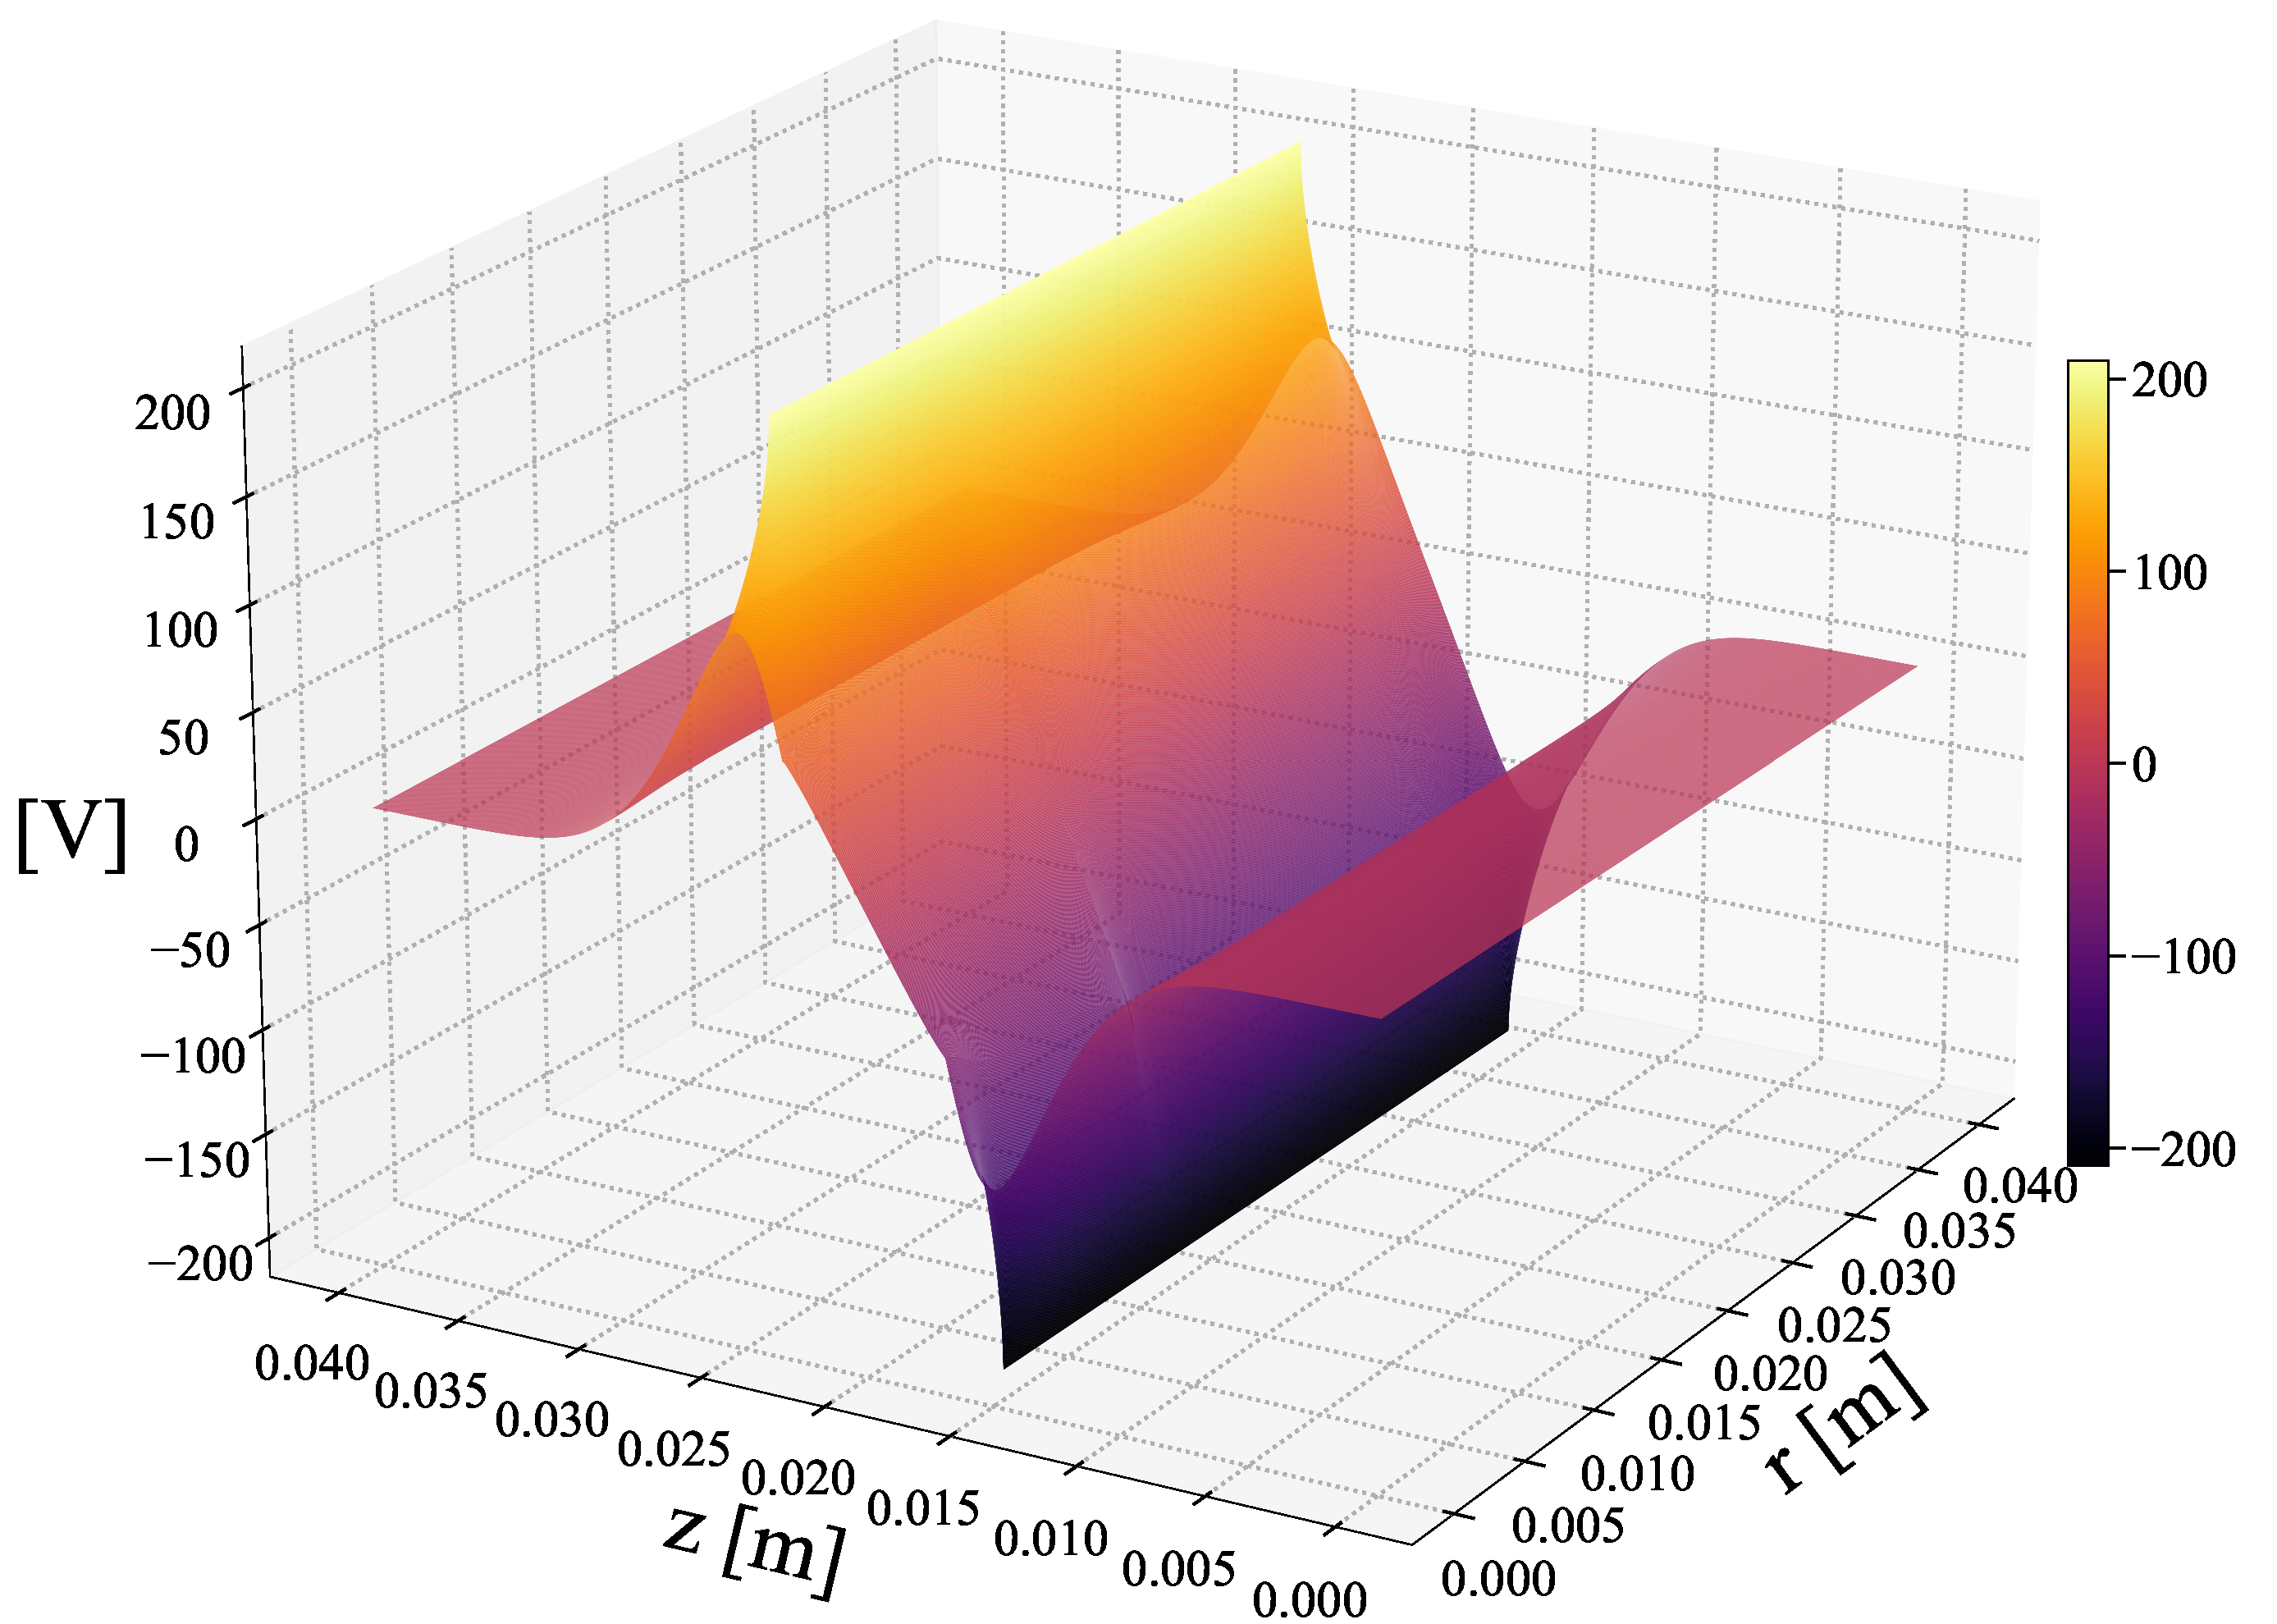
\includegraphics[width=\textwidth]{ALGAAS/assembly1_sim.pdf}
  \caption{Numerically computed potential map estimate ($V(z,r)$ in cylindrical coordinates)}
  \label{fig:poissoncalcoutput}
\end{figure}

The computed $E_z$ screened by the coating at $r = 0$ for $V = 1$ is estimated to be 42 $[\mathrm{V}/\mathrm{m}]$ and will be included in the calibration as a pockels cell field conversion factor $42 [(\mathrm{V} / \mathrm{m}) / \mathrm{V}]$  

\subsubsection{Voltage drive electronics}
\begin{figure}[H]
    \includegraphics[width=\textwidth]{ALGAAS/13-Sep-2021_e_field_inside_outside_normal.pdf}
    \caption{The availablility of required voltage amplifiers during the course of this study was limited and lead to the use of multiple high voltage amplifiers with all transfer functions listed.}
\label{fig:Ez}
\end{figure}


\begin{figure}[H]
    \includegraphics[width=\textwidth]{ALGAAS/tfs/hva_compare.pdf}
    \caption{Different high voltage amplifier transfer functions used for the study}
    \label{fig:hvacompare}
\end{figure}

\subsection{Servo Overview}
\begin{figure}[!ht]
	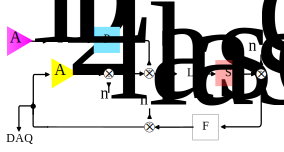
\includegraphics[width=\textwidth]{figs/ALGAAS/pock_control_diagram.pdf}
	\caption{A controls diagram of the designed servo.}
	\label{fig:pock_control_servo}
\end{figure}

\subsection{Calibration}

The Electric field coupling can be expressed as a measured voltage:
$$\mathrm{V} = \frac{1}{1 + \mathrm{G}} \nu_\mathrm{laser} - \frac{\mathrm{G}}{1 + \mathrm{G}} \mathrm{C} \mathrm{E} \mathrm{A}_{2} \mathrm{V}_\mathrm{in} - \frac{\mathrm{F} \mathrm{A}_1}{1 + \mathrm{G}} \nu_\mathrm{S} - \frac{A_1}{1 + \mathrm{G}} \nu_\mathrm{F}$$
With G representing the open loop gain ($\mathrm{G} = \mathrm{A}_1 \mathrm{F} \mathrm{S} \mathrm{L}$). The feedback signal transforms into:

$$ \mathrm{V}_\mathrm{out} = \mathrm{F} \mathrm{S} \mathrm{L} (\mathrm{V} + \mathrm{C} \mathrm{E} \mathrm{A}_{2} \mathrm{V}_\mathrm{in}) + \mathrm{F} \nu_\mathrm{S} + \nu_\mathrm{F} = \frac{\mathrm{F} \mathrm{S} \mathrm{L}}{1 + } \mathrm{C} \mathrm{E} \mathrm{A}_{2} \mathrm{V}_\mathrm{in}
$$
$$ \mathrm{V}_\mathrm{out} = \mathrm{F} \mathrm{S} \mathrm{L} (\mathrm{V} + \mathrm{C} \mathrm{E} \mathrm{A}_{2} \mathrm{V}_\mathrm{in}) + \mathrm{F} \nu_\mathrm{S} + \nu_\mathrm{F} = \frac{\mathrm{F} \mathrm{S} \mathrm{L}}{ 1 + \mathrm{G}} \mathrm{C} \mathrm{E} \mathrm{A}_{2} \mathrm{V}_\mathrm{in} + \frac{\mathrm{F} \mathrm{S} \mathrm{L}}{ 1 + \mathrm{G}} \nu_\mathrm{laser} + \frac{\mathrm{F} }{ 1 + \mathrm{G}} \nu_\mathrm{S} +  \frac{1}{ 1 + \mathrm{G}} \nu_\mathrm{F}$$ 
Therefore, the transfer function ($\frac{\mathrm{V}_\mathrm{out}}{\mathrm{V}_\mathrm{in}}$) : 
$$ \frac{\mathrm{V}_\mathrm{out}}{\mathrm{V}_\mathrm{in}} = \frac{\mathrm{F} \mathrm{S} \mathrm{L}}{1 + \mathrm{G}}\mathrm{C} \mathrm{E} \mathrm{A}_{2}  + \frac{\mathrm{F} \mathrm{S} \mathrm{L}}{ 1 + \mathrm{G}} \frac{\nu_\mathrm{laser}}{\mathrm{V}_\mathrm{in}}+ \frac{\mathrm{F} }{ 1 + \mathrm{G}} \frac{\nu_\mathrm{S}}{\mathrm{V}_\mathrm{in}} +  \frac{1}{ 1 + \mathrm{G}} \frac{\nu_\mathrm{F}}{\mathrm{V}_\mathrm{in}}$$
If the induced excitation is larger than the noise we can approximate the last equation:

$$ \frac{\mathrm{V}_\mathrm{out}}{\mathrm{V_{in}}} \approx \frac{\mathrm{F} \mathrm{S}\mathrm{L}}{1 + \mathrm{G}} \mathrm{C} \mathrm{E} \mathrm{A}_{2} = \frac{\mathrm{G}}{1 + \mathrm{G}} \mathrm{C} \mathrm{E} \frac{\mathrm{A}_{2}}{\mathrm{A}_{1}} $$
 

\iffalse
The calibration math for this measurement explicitly starts with what I
call \(\alpha(f)\) which is a vector of complex numbers that represents
the transfer function \(\mathrm{CH2}(f)/\mathrm{CH1}(f)\) where:

\[\mathrm{CH1}(f) = \mathrm{Source}(f)\] and
\[\mathrm{CH2}(f) = \frac{\mathrm{S}(f)* signal(f)}{1-\mathrm{OLG}(f)}\]

Where \[\mathrm{OLG}(f) = \mathrm{A}(f)* \mathrm{S}(f)\]

and \(signal(f)\) is the demodulated output from
\(\mathrm{RFPD}_\mathrm{refl}\) and \(\mathrm{S}(f)\) is the transfer
function of the frequency stabilization servo.

From here we solve for signal(f):

\[signal(f) = \mathrm{CH2}(f) * \mathrm{A}_{1}(f) * \mathrm{A}_2* \frac{(1-\mathrm{OLG}(f))}{\mathrm{OLG}(f)}\]

Where \(\mathrm{A}_{1}(f)\) informs the frequency dependent drive sent
to the laser PZT to keep the cavity locked and \(\mathrm{A}_2\) is the
laser frequency detuning factor {[}Hz/V{]} (can be estimated from
measuring PDH).

Currently \(signal(f)\) provides a frequency noise spectra which then
can be converted into a displacement spectra with the following
relation:

\[\frac{\Delta f}{f_\mathrm{laser}} = \frac{\Delta L}{L_\mathrm{cav}}\]

This allows us to imagine the frequency noise spectra as a length noise
spectra due to the drive on the electrodes:

\[signal(f) = \alpha(f)* \mathrm{Source}(f) * \mathrm{A}_{1}(f) * \mathrm{A}_2* \frac{(1-\mathrm{OLG}(f))}{\mathrm{OLG}(f)} * \frac{L_\mathrm{cav}}{f_\mathrm{laser}}\hspace{35pt} [m_\mathrm{pk}]\]

And for the measurement normalized by the drive voltage on the
electrodes:

\[\frac{signal(f)}{\mathrm{Source}(f) * \mathrm{G}(f)} = \frac{\alpha(f)}{\mathrm{G}(f)} * \mathrm{A}_{1}(f) * \mathrm{A}_2* \frac{(1-\mathrm{OLG}(f))}{\mathrm{OLG}(f)} * \frac{L_\mathrm{cav}}{f_\mathrm{laser}}\hspace{35pt} \bigg[\frac{m_\mathrm{pk}}{V_\mathrm{pk}}\bigg]\]
\#\# Noise or single frequency drive measurement : \(n(f)\) The
calibration math for this measurement is essentially equivalent to the
transfer function measurement above. The only difference is:

\[\mathrm{CH1}(f) = \frac{\mathrm{S}(f)* signal(f)}{1-\mathrm{OLG}(f)}\]

and

\[signal(f) = \mathrm{CH1}(f) * \mathrm{A}_{1}(f) * \mathrm{A}_2* \frac{(1-\mathrm{OLG}(f))}{\mathrm{OLG}(f)} * \frac{L_\mathrm{cav}}{f_\mathrm{laser}}\]

Where \(signal(f)\) in this measurement represents the free running
cavity displacement noise with the exception of a single frequency if it
is not a noise measurement.

If \(\mathrm{CH1}(f)\) is in \(\frac{V_\mathrm{rms}}{\sqrt{Hz}}\) then
signal(f) will be in \(\frac{m_\mathrm{rms}}{\sqrt{Hz}}\)

or

If \(\mathrm{CH1}(f)\) is in \(V_\mathrm{pk}\) then signal(f) will be in
\(m_\mathrm{pk}\) 
\fi

%\#\# Calibration code
%The error signal spectra probed at the FSS:
%\begin{equation}
%\mathrm{VFSSOUT}_\mathrm{rms}/\sqrt{Hz} \rightarrow m_\mathrm{rms}/\sqrt{\mathrm{Hz}}
%\end{equation}
%With the known frequency response of the servo electronics, we \autoref{sec:calibration} the measurement into differential length:
%\begin{equation}
%	\Delta \mathrm{L} = \mathrm{source}*\alpha(f) \mathrm{A}(f)*\frac{1+\mathrm{OLG}(f)}{\mathrm{OLG}(f)}*\frac{\mathrm{L_{cav}}}{f_\mathrm{laser}} \quad \big[ m_\mathrm{pk} / \sqrt{Hz} \big]
%\end{equation}
\section{Results}
Significant barriers were encountered in the form of cavity differential length noise especially when mounting the optics in accessible non-conductive materials. Firstly, most commercial optical mounts are constructed with conductive materials which proves problematic when working to isolate the coating from non-normal field gradients within the coating volume of interest. For this reason, efforts were focused on developing a suitable mounting solution that would provide adequate isolation from any uncontrolled field magnitudes while driving a field normally incident on the surface with enough strength and uniformity across the beam area to extract a measurement of the differential length change from the Pockels effect. The mounts studied span different geometries and different material properties. The varying geometrical assemblies rendered various responses and for this reason some discussions will be divided accordingly. The most stable solution revealed that ringing of the sample acoustic modes may be responsible For reassurance, we compare displacement spectra against that of a nearly identical cavity with a flat non-crystalline mirror coating to perform a null measurement reference; ruling out the Pockels effect and providing information for noise investigations.


\subsection{Mounting Strategies}
The following section details measurements performed with various longitudinal pockel cell mounts. Further details (assembly parameters, blueprints, and visual aids) can be found in the appendix.

\subsubsection{Assembly 1}

\begin{figure}[!ht]
    \begin{subcaptiongroup}
	    \includegraphics[width=.5\textwidth]{figs/ALGAAS/assemblies/assembly1/assembly1_dissassembled.pdf}
	    \phantomcaption\label{A1disassembled}
	    \includegraphics[width=.5\textwidth]{figs/ALGAAS/assemblies/assembly1/assembly1_flaw.pdf}
	    \phantomcaption\label{A1flaw}
    \end{subcaptiongroup}
    \caption{Assembly 1 was constructed to meet two criteria: the same solution of housing the sample and electrodes as Assembly 0, but also offer pitch / yaw control via an ortho-planar spring design (Brigham Young University).}
    \label{fig:A1pt0}
\end{figure}
\FloatBarrier


The construction revealed flaws; made most obvious when comparing to displacement noise of traditional optical mounts. Pitch and yaw control via the ortho-planar spring were prioritized to avoid metal springs and further mount pieces. The solution became unjustifiable when observing the the displacement noise coupling from the mount.

%%Re-run this calibration with adequate voltage normalization for a response unit [$m_\mathrm{pk} / [V / m]$]

\begin{figure}[H]
\centering
\includegraphics[width=\textwidth]{figs/ALGAAS/assemblies/assembly1/assembly1_2_compare_standmount.pdf}
\caption{Measured displacement spectra for Assembly 1.2 of the longitudinal pockels cell mount compared to the standard kinematic mount. Both measurements were recorded with the the CVI Melles-Griot (amorphous) mirror coating sample installed in the assembly.}
%%Units and legend labels need increase in font size. Remove Swept sine measurement title.
\label{fig:A12cmpkinmnt}
\end{figure}


Attempts at improving the pitch dithering were tried with side set screws but mostly caused significant misalignment (less power in fundamental mode, locking issues, etc.). This lead to the final alternative for this assembly type; with the same PLA stack indicated in ~\hyperref[fig:A1pt0]{Assembly 1}.

\begin{figure}[!ht]
	\begin{subcaptiongroup}
		\includegraphics[width=.5\textwidth]{figs/ALGAAS/assemblies/assembly1/assembly1_mod_front.pdf}
		\phantomcaption\label{A1front}
		\includegraphics[width=.5\textwidth]{figs/ALGAAS/assemblies/assembly1/assembly1_mod_side.pdf}
		\phantomcaption\label{A1side}
	\end{subcaptiongroup}
    \caption{A modification implemented  with the intention of reducing pitch dithering while still having control of DC YAW}
    \label{fig:A1pt0mod}
\end{figure}

\begin{figure}[H]
    \includegraphics[width=\textwidth]{figs/ALGAAS/results_figs/assembly1/1_2_algaas_tfwcmb.pdf}
    \caption{Assembly 1.2 and 1.3 transfer function measurement and separate noise displacement spectra measurement with the $\gaas$/$\algaas$ sample installed. Measurements were taken from 3kHz up to 21kHz on using a Stanford Research 785 spectrum analyzer.}
    \label{fig:assembly12and13displacementspectraalgaas}
\end{figure}

\begin{figure}[H]
    \includegraphics[width=\textwidth]{figs/ALGAAS/results_figs/assembly1/1_2_cvi_compare_tfwcmb.pdf}
    \caption{Assembly 1.2 and 1.3 transfer function measurement and separate noise displacement spectra measurement with a CVI Melles Griot flat mirror sample ($R \approx $ sample installed. Measurements were taken from 1kHz up to 30kHz on using a Stanford Research 785 spectrum analyzer.}
    \label{fig:assembly12and13displacementspectracvi}
\end{figure}

\subsubsection{Assembly 2}

With considerations after Assembly 1, a more monolithic optical mount design with a simple geometry was imagined. PLA material compliance factoring to the seen drive noise. To see if it could be due to the compliance of the assembly material or printing, we tested this assembly design against different infills of PLA, PETG, and a version machined from solid PVC. With this modification, came also a different plate geometry. The assumption is the region of interest of the injection would not be heavily influenced by the non-circular plate geometry where it matters.

% Some citations:
%\cite{PINTO2015635}

%\begin{figure}[!ht]
%	\begin{subcaptiongroup}
%		\includegraphics[width=.5\textwidth]{figs/ALGAAS/assemblies/assembly2/assembly2_PVC.pdf}
%		\phantomcaption\label{A2_PVC}
%		\includegraphics[width=.5\textwidth]{figs/ALGAAS/assemblies/assembly2/assembly2_PVC.pdf}
%		\phantomcaption\label{A2_PVC}
%    	\end{subcaptiongroup}
%    \caption{An iteration of assembly 2 comprised of a PVC mount with two rectangular (1.1"X2") plates with a central aperture of 3mm}
%    \label{fig:assembly2}
%\end{figure}

\begin{figure}[H]
    \includegraphics[width=\textwidth]{figs/ALGAAS/results_figs/assembly2/2_0_compare_1_1.pdf} 
    \caption{Assembly 2.0 transfer function measurements compared to Assembly 1.1, Measurements were taken from 1kHz up to 30kHz on using a Stanford Research 785 spectrum analyzer.}
    \label{fig:assembly2and1one}
\end{figure}


\begin{figure}[H]
    \includegraphics[width=\textwidth]{figs/ALGAAS/results_figs/assembly2/vary_da.pdf}
    \caption{The varied drive amplitudes input into the HVA to perform the following test}
    \label{fig:varyda}
\end{figure}

\begin{figure}[H]
    \includegraphics[width=\textwidth]{figs/ALGAAS/results_figs/assembly2/vv53.pdf} 
    \caption{Assembly 2.0 transfer function measurements with varied drive amplitudes indicated in ~\autoref{fig:varyda}.}
    \label{fig:vv53}
\end{figure}


\begin{figure}[H]
    \includegraphics[width=\textwidth]{figs/ALGAAS/results_figs/assembly2/vary_daao.pdf}
    \caption{The varied drive amplitudes and offsets input into the HVA to perform the following test}
    \label{fig:varydaao}
\end{figure}

\begin{figure}[H]
    \includegraphics[width=\textwidth]{figs/ALGAAS/results_figs/assembly2/vvao517.pdf} 
    \caption{Assembly 2.0 transfer function measurements with varied drive amplitudes and offsets indicated in ~\autoref{fig:varydaao}.}
    \label{fig:vvao517}
\end{figure}

\subsubsection{Assembly 3 (MACOR mount)}
With most of the same characteristics from Assembly 3, an optical mount made of MACOR, a machinable ceramic, was constructed and installed. With the material's high Young's modulus (66.9 GPa), and a moderate Poisson ratio (.29) \cite{macor} making it by far the most durable / non-conductive mounting solution tried.

An optical mount for the sample made with MACOR, along with spherical glass bearnings with a .48 $\pm$ .01 cm $\diameter$, and a McMaster-Carr 8-32, 1/2" ceramic screw were used to clamp the optical sample within a bored 25.74 $\pm$ .5 mm $\diameter$ barrel. Two 1.24" $\diameter$ holes were also bored at a 9 mm depth about the front and back side of the optical mount to accomodate for a flush fit of copper electrodes. The construction suggests a 1 $\pm$ .5 mm clearance between the front and back surface of the sample to the electrode plates.

%%FIGURE: sample in-situ
\begin{figure}[!ht]
    \begin{subcaptiongroup}
	    \includegraphics[width=.5\textwidth]{figs/ALGAAS/assemblies/assembly3/assembly3_disassembled.pdf}
	    \phantomcaption\label{subfig:A3disassembled}
	    \includegraphics[width=.5\textwidth]{figs/ALGAAS/assemblies/assembly3/assembly3_isometric.pdf}
	    \phantomcaption\label{subfig:A3isometric}
    \end{subcaptiongroup}
    \caption{Assembly 3: \subref{subfig:A3disassembled} disassembled configuration and \subref{subfig:A3isometric} an isometric view of the assembled configuration.}
    \label{fig:assembly3}
\end{figure}


\begin{figure}[H]
    \includegraphics[width=\textwidth]{figs/ALGAAS/results_figs/assembly3/petgmsvv64.pdf}
    \caption{A polarization depdendent test using the MACOR mount}
    \label{fig:measurementsum}
\end{figure}

\subsubsection{Acousto-optical coupling}
Drive coupling seec in the transfer function measurements with the MACOR mounts appeared consistent. Varying the mechanical configurations (i.e. differential electrode and / or optic set screw settings) to the slightest degree left us to discover a mechanical action via the excitations from the sample-mount acoustic modes from the construction are rung when driving the voltage on electrodes plates. Tracking consistent mechanical action for assemblies prior to Assembly 3 were difficult due to inconsistencies in mechanical settings between some measurements. When more consistency was realized (i.e. utilizing a MACOR mount and careful tracking of the sample set screw torque), it was more transparent that the sample-mount acoustic modes were responsible with similar features between the $\gaas$/$\algaas$ coating and the non-crystalline HR coating from ATFilms. The cleanest versions of these measurements with coorespondence of FEA suggest the acousto-optical modes with highest contributions of cavity length noise at regions below 10 kHz and 40 kHz - 80 kHz. 

%\begin{itemize}
%\item \textbf{Vibration of plates (Leissa)} \cite{leissa:1969} Computing frequencies and order of magnitude
%	\begin{itemize}
%	    \item Numerical computation (Order of magnitude result)
%	\end{itemize}
%\item \textbf{Steve's COMSOL model results}
%\end{itemize}

\subsection{Conclusion}
The significantly improved thermal noise performance of $\gaas$/$\algaas$ HR coatings make these crystalline coatings a prime candidate for the core optics in current and future gravitational wave detectors. The measured upper threshold of the electro-optic noise is demonstrated to be $\sim 10^{-24} \; [1/\sqrt{\mathrm{Hz}}]$ two orders of magnitude below the designed noise floor $\sim 10^{-26}\; [1/\sqrt{\mathrm{Hz}}]$ of current and future gravitational wave detectors.
